% changelog: "1.0.0, 2024-08-18, Approvazione per PB"
\documentclass[8pt]{article}
\usepackage[italian]{babel}
\usepackage[utf8]{inputenc}
\usepackage[letterpaper, left=1in, right=1in, bottom=0.75in, top=0.75in]{geometry}
\usepackage{amsmath}
\usepackage{subfiles}
\usepackage{lipsum}
\usepackage{csquotes}
\usepackage{amsfonts}
\usepackage[sfdefault]{plex-sans}
\usepackage{float}
\usepackage{pifont}
\usepackage{mathabx}
\usepackage[euler]{textgreek}
\usepackage{makecell}
\usepackage{tikz}
\usepackage{wrapfig}
\usepackage{siunitx}
\usepackage{amssymb} 
\usepackage{tabularx}
\usepackage{adjustbox}
\usepackage[document]{ragged2e}
\usepackage{floatflt}
\usepackage[hidelinks]{hyperref}
\usepackage{graphicx}
\usepackage{hyperref}
\setcounter{tocdepth}{4}
\usepackage{caption}
\usepackage{multicol}
\usepackage{tikz}
\setlength\parindent{0pt}
\captionsetup{font=footnotesize}
\usepackage{fancyhdr} 
\usepackage{graphicx}
\usepackage{capt-of}% 
\usepackage{booktabs}
\usepackage{varwidth}
\usepackage{datetime2}
\usepackage{xcolor}
\usepackage{longtable}
\usepackage{array}
\usepackage{ragged2e}
\usepackage{colortbl}
\usepackage{verbatim}
\usepackage{enumitem}

\newcommand{\customtitle}{MANUALE UTENTE}% o ESTERNO

% -- STILE COLONNA CENTRATA PER TABELLE -- %
\newcolumntype{M}[1]{>{\centering\arraybackslash}m{#1}}

% -- STILE INTESTAZIONE -- %
\fancypagestyle{mystyle}{
	\fancyhf{} 
	\fancyhead[R]{
\includegraphics[height=1cm]{../../template/images/logos/NaN1fy_logo.png}} 
	\fancyhead[L]{\leftmark} 
	\renewcommand{\headrulewidth}{1pt} 
	\fancyhead[L]{\customtitle} 
	\renewcommand{\headsep}{1.3cm} 
	\fancyfoot[C]{\thepage} 
}

% -- PER LA FIRMA -- %
\newcommand{\signatureline}[1]{%
	 \par\vspace{0.5cm}
	\noindent\makebox[\linewidth][r]{\rule{0.2\textwidth}{0.5pt}\hspace{3cm}\makebox[0pt][r]{\vspace{3pt}\footnotesize #1}}%
}

% -- PER IL GLOSSARIO -- %
\newcommand{\glossterm}[1]{#1\textsuperscript{G}} % inserisci \glossterm{termine}

% -- per abilitare 4x sottosezioni es 2.1.1.1
\setcounter{secnumdepth}{4}
\newcommand{\subsubsubsection}[1]{\paragraph{#1}\mbox{}\\\\}

\begin{document}
\definecolor{myblue}{RGB}{23,103,162}
\begin{titlepage}
	\begin{tikzpicture}[remember picture, overlay]
		\node[anchor=south east, opacity=0.2, yshift = -4cm, xshift= 2em] at (current page.south east) {
\includegraphics[width=0.7\textwidth, trim=0cm 0cm 5cm 0cm, clip]{../../template/images/logos/Universita_Padova_transparent.png}}; 
		\node[anchor=north west, opacity=1, yshift = 4.2cm, xshift= 1.4cm, scale=1.6] at (current page.south west) {
\includegraphics[width=4cm]{../../template/images/logos/NaN1fy_logo.png}};
	\end{tikzpicture}
	
	\begin{minipage}[t]{0.47\textwidth}
		{\large{\textsc{Destinatari}}
			\vspace{3mm}
			\\ \large{\textsc{Prof. Tullio Vardanega}}
			\\ \large{\textsc{Prof. Riccardo Cardin}}
		}
	\end{minipage}
	\hfill
	\begin{minipage}[t]{0.47\textwidth}\raggedleft
		{\large{\textsc{Redattori}}
			\vspace{3mm}
			{\\\large{\textsc{Davide Donanzan}\\}} % massimo due 
			{\large{\textsc{Veronica Tecchiati}}}
			
			
		}
		\vspace{8mm}
		
		{\large{\textsc{Verificatori}}
			\vspace{3mm}
			{\\\large{\textsc{Veronica Tecchiati}\\}} 
			{\large{\textsc{Pietro Busato}\\}} 
			{\large{\textsc{Oscar Konieczny}\\}}
			
		}
		\vspace{2mm}\vspace{2mm}
	\end{minipage}
	\vspace{4cm}
	\begin{center}
		\begin{flushright}
			{\fontsize{30pt}{52pt}\selectfont \textbf{Manuale Utente}} % o ESTERNO
		\end{flushright}
		\vspace{3cm}
	\end{center}
	\vspace{10 cm}
	{\small \textsc{\href{mailto: nan1fyteam.unipd@gmail.com}{nan1fyteam.unipd@gmail.com}}}
\end{titlepage}
\pagestyle{mystyle}
\section*{Registro delle Modifiche}
\begin{table}[ht!]	
	\centering
	\begin{tabular}{p{1.2cm} p{2cm} p{5cm} p{3cm} p{3cm}}
		\toprule
		\textbf{Versione}& \textbf{Data} & \textbf{Descrizione} & \textbf{Redattore} & \textbf{Verificatore} \\
		\midrule
            1.0.0 & 2024-08-18 & \textbf{Approvazione per PB} & & \\\\
            0.1.0 & 2024-08-10 & Stesura sezioni \ref{sec:requirements} e \ref{sec:instructions}. & Veronica Tecchiati & Pietro Busato \\\\
		    0.0.0 & 2024-07-01 & Stesura struttura e sezioni \ref{sec:intro} e \ref{sec:support}. & Davide Donanzan & Veronica Tecchiati \\
		\bottomrule
		% Ruolo Redattore o Verificatore
	\end{tabular}
	\caption*{Tabella: Registro delle modifiche.}
	\label{table:Registro delle modifiche}
\end{table}
\newpage
\tableofcontents
\newpage
\listoffigures
\newpage
%\listoftables
\newpage
\justifying
\section{Introduzione}\label{sec:intro}
\subsection{Scopo del documento}
Il presente manuale è concepito per fornire un supporto agli utenti nell’utilizzo efficace del software, 
consentendo loro di sfruttare appieno tutte le sue \glossterm{funzionalità}, al fine di garantire un’esperienza ottimale.
In tal modo, si vuole informare l’amministratore pubblico dei requisiti minimi da soddisfare per
poter usufruire del prodotto, degli step necessari per la sua installazione e di tutte le funzionalità a sua disposizione.
 Poiché l’installazione del software è gestita da personale tecnico specializzato, questo
 manuale non include istruzioni dettagliate per l’installazione, bensì si concentra piuttosto sui
 passaggi necessari per utilizzare il software una volta installato correttamente.
\subsection{Scopo del prodotto}
L'obiettivo del progetto ``SyncCity: \glossterm{Smart City} Monitoring Platform" è quello di creare una piattaforma atta al monitoraggio
di \glossterm{sensori} geograficamente distribuiti nel territorio di una città. I sensori in questione
permettono la misurazione e segnalazione di dati in \glossterm{real-time} riguardanti le più disparate
caratteristiche e necessità del territorio, quali temperatura ed umidità esterna, occupazione di
stalli di parcheggio, funzionamento o guasto elettrico di colonnine di ricarica, traffico stradale e via
dicendo. La \glossterm{Proponente} richiede la simulazione di alcuni dei sensori nominati nonchè la
gestione dei dati, della loro persistenza e della loro rappresentazione grafica attraverso \glossterm{widget} e
grafici. 
\\\\SyncCity permetterà un miglioramento della \glossterm{qualità} dei servizi offerti dalla città attraverso il continuo monitoraggio della stessa, ottenendo, gestendo e successivamente condividendo i dati con gli utenti. 
% \subsection{Accesso alla piattaforma}
\subsection{Glossario}
Per garantire chiarezza nel linguaggio utilizzato nei documenti, è stato redatto un Glossario contenente le definizioni dei termini con significato specifico da disambiguare. Tali termini sono contrassegnati con una G ad apice. L'inserimento di un termine nel Glossario è considerato completo solo dopo averne fornito la definizione.
\subsection{Riferimenti}
\subsubsection{Normativi}
\begin{itemize}
	\item \textit{Norme di Progetto v2.0.0};
	\item Presentazione e documentazione del \glossterm{capitolato} d’appalto C6 - SyncCity:
	\begin{itemize}
 \setlength\itemsep{0em}
		\item \href{https://www.math.unipd.it/~tullio/IS-1/2023/Progetto/C6p.pdf}{\color{myblue}https://www.math.unipd.it\textasciitilde{}tullio/IS-1/2023/Progetto/C6p.pdf} (Ultimo accesso: \today)
		\item \href{https://www.math.unipd.it/~tullio/IS-1/2023/Progetto/C6.pdf}{\color{myblue}https://www.math.unipd.it/\textasciitilde{}tullio/IS-1/2023/Progetto/C6.pdf} (Ultimo accesso: \today)
	\end{itemize}
	\item Regolamento di progetto:
	\begin{itemize}
		\item \href{https://www.math.unipd.it/~tullio/IS-1/2023/Dispense/PD2.pdf}{\color{myblue}https://www.math.unipd.it/\textasciitilde{}tullio/IS-1/2023/Dispense/PD2.pdf} (Ultimo accesso: \today)
	\end{itemize}
\end{itemize}
% \clearpage
\subsubsection{Informativi}
\begin{itemize}
\setlength\itemsep{0em}
    \item \textit{Analisi dei Requisiti v2.0.0};
    \item \textit{Glossario v2.0.0};
    \item \textit{Specifica Tecnica v1.0.0};
\end{itemize}
\clearpage
\section{Requisiti minimi} \label{sec:requirements}
Per garantire il corretto funzionamento del prodotto è necessario soddisfare i requisiti minimi descritti di seguito.
\subsection{Requisiti hardware}
Essendo SyncCity un applicativo web, non è richiesto l'utilizzo di dispositivi con prestazioni hardware particolarmente elevate. Le seguenti specifiche sono dunque sufficienti a garantire un'esperienza utente soddisfacente e completa:  
\begin{itemize}
\setlength\itemsep{0em}
    \item \textbf{Processore:} Quad-Core 2.4 GHz 64 bit;
    \item \textbf{RAM:} 6 GB;
    \item \textbf{Spazio libero su disco:} 6 GB;
    \item \textbf{Connessione a internet:} stabile.
\end{itemize}
\subsection{Requisiti di sistema operativo}
L'applicativo può essere eseguito su diversi sistemi operativi. Di seguito sono indicate le versioni dei più comuni sistemi operativi che consentono di utilizzare correttamente SyncCity:
\begin{itemize}
\setlength\itemsep{0em}
    \item \textbf{Windows:} 10 o 11 con WSL 2;
    \item \textbf{MacOS:} 11.0 Big Sur;
    \item \textbf{Linux:}
    \begin{itemize}
        \item Ubuntu: 22.04;
        \item Debian: 12;
        \item Fedora: 38;
        \item RHEL: 8.
    \end{itemize}
\end{itemize}
Si noti che l'applicazione può essere eseguita anche su sistemi operativi differenti da quelli indicati o meno aggiornati, tuttavia non è garantito un supporto completo.
\subsection{Requisiti browser}
Essendo SyncCity un applicativo web, è richiesto l'utilizzo di un browser per la sua fruizione. Si riportano di seguito le versioni dei più comuni browser web che garantiscono il corretto funzionamento del prodotto:
\begin{itemize}
\setlength\itemsep{0em}
    \item \textbf{Google Chrome:} v124;
    \item \textbf{Mozilla Firefox:} v125;
    \item \textbf{Microsoft Edge:} v123;
    \item \textbf{Safari:} v17.4;
\end{itemize}
Si noti che l'applicazione può essere eseguita anche su browser differenti da quelli indicati o meno aggiornati, tuttavia non è garantito un supporto completo.
\newpage
\section{Istruzioni all'uso} \label{sec:instructions}
\setlength\parindent{0pt}
\subsection{Login}
All'avvio del prodotto, l'utente visualizza una schermata di login che espone due campi di inserimento, ``Email o username" e ``Password". L'utente può quindi digitare nei campi corrispondenti le proprie credenziali e cliccare sul pulsante ``Log in" per ottenere l'accesso al sistema. 
\begin{figure}[H]
    \centering
    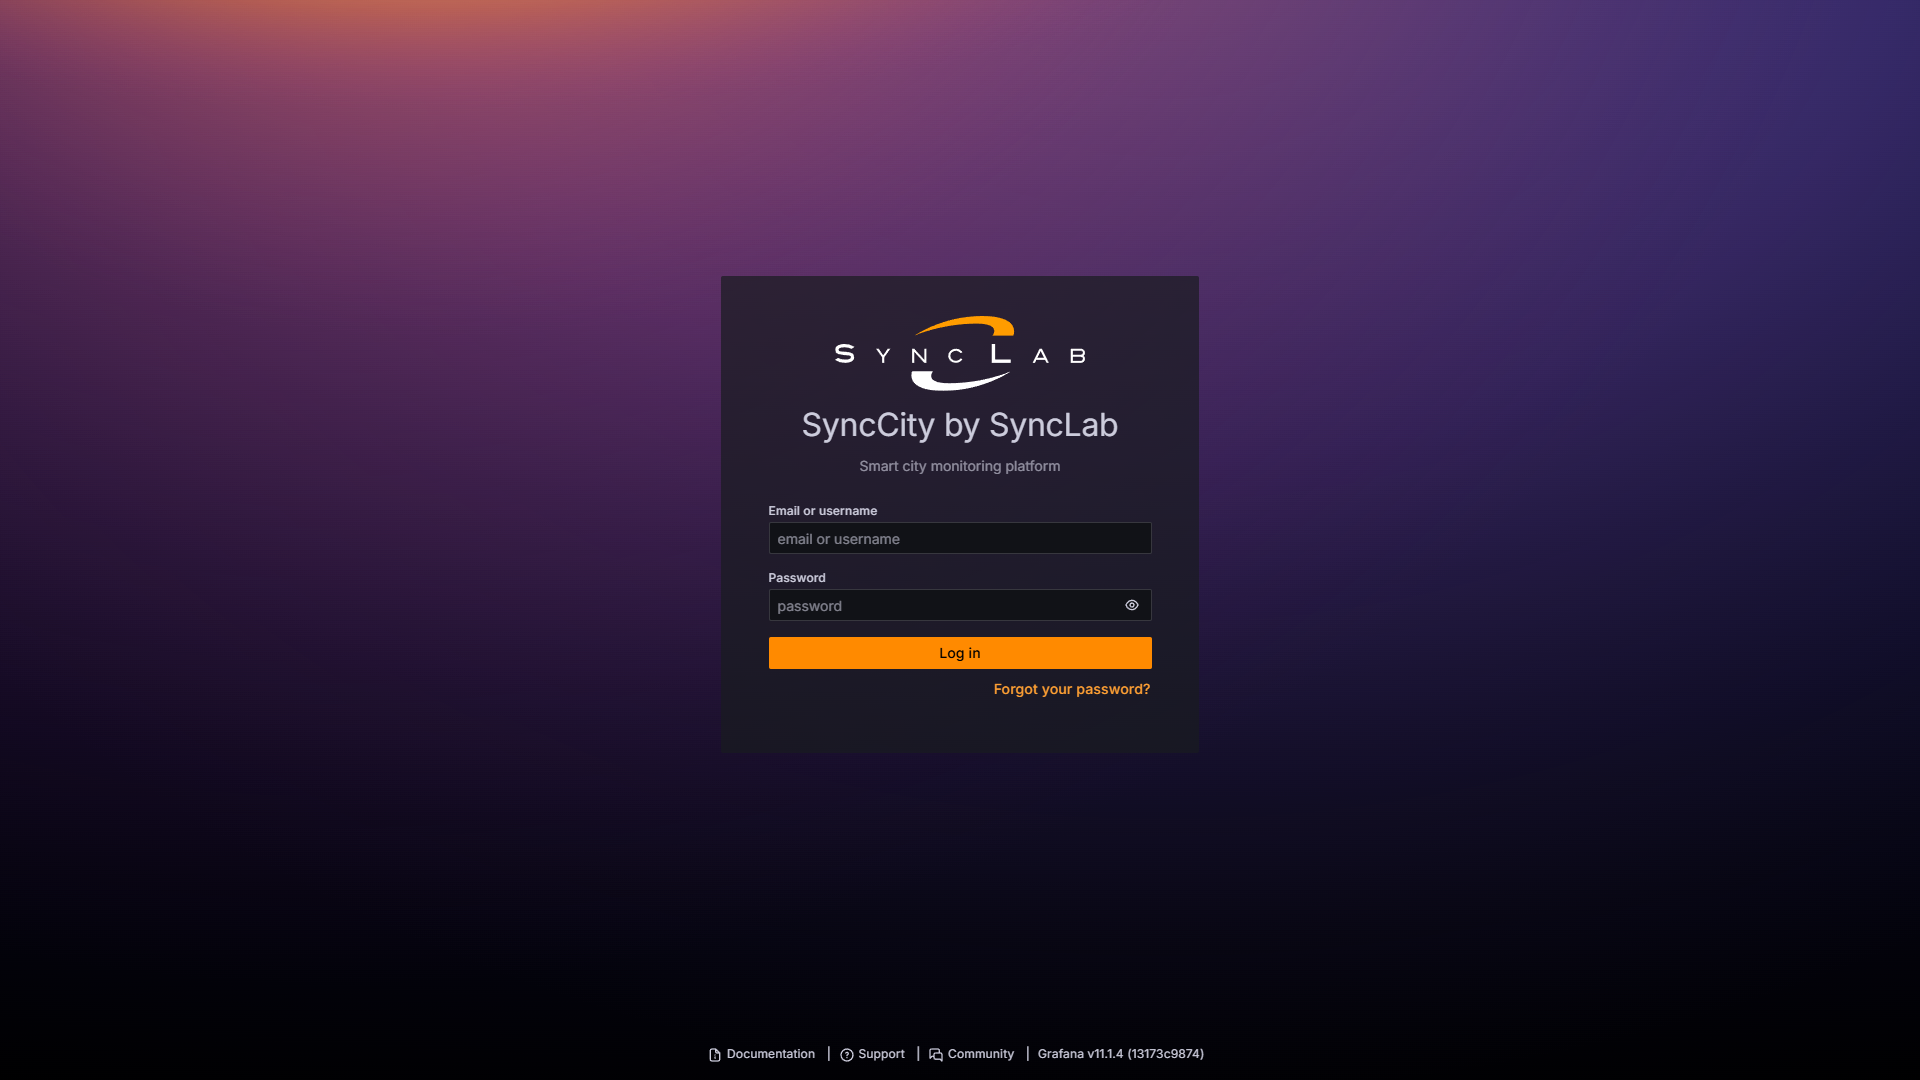
\includegraphics[width=15cm]{./images_mu/login.png}
    \caption{Schermata di login.}
    \label{figure:Schermata di login.}
\end{figure}
Qualora le credenziali inserite fossero errate verrà visualizzato un messaggio di errore.
\begin{figure}[H]
    \centering
    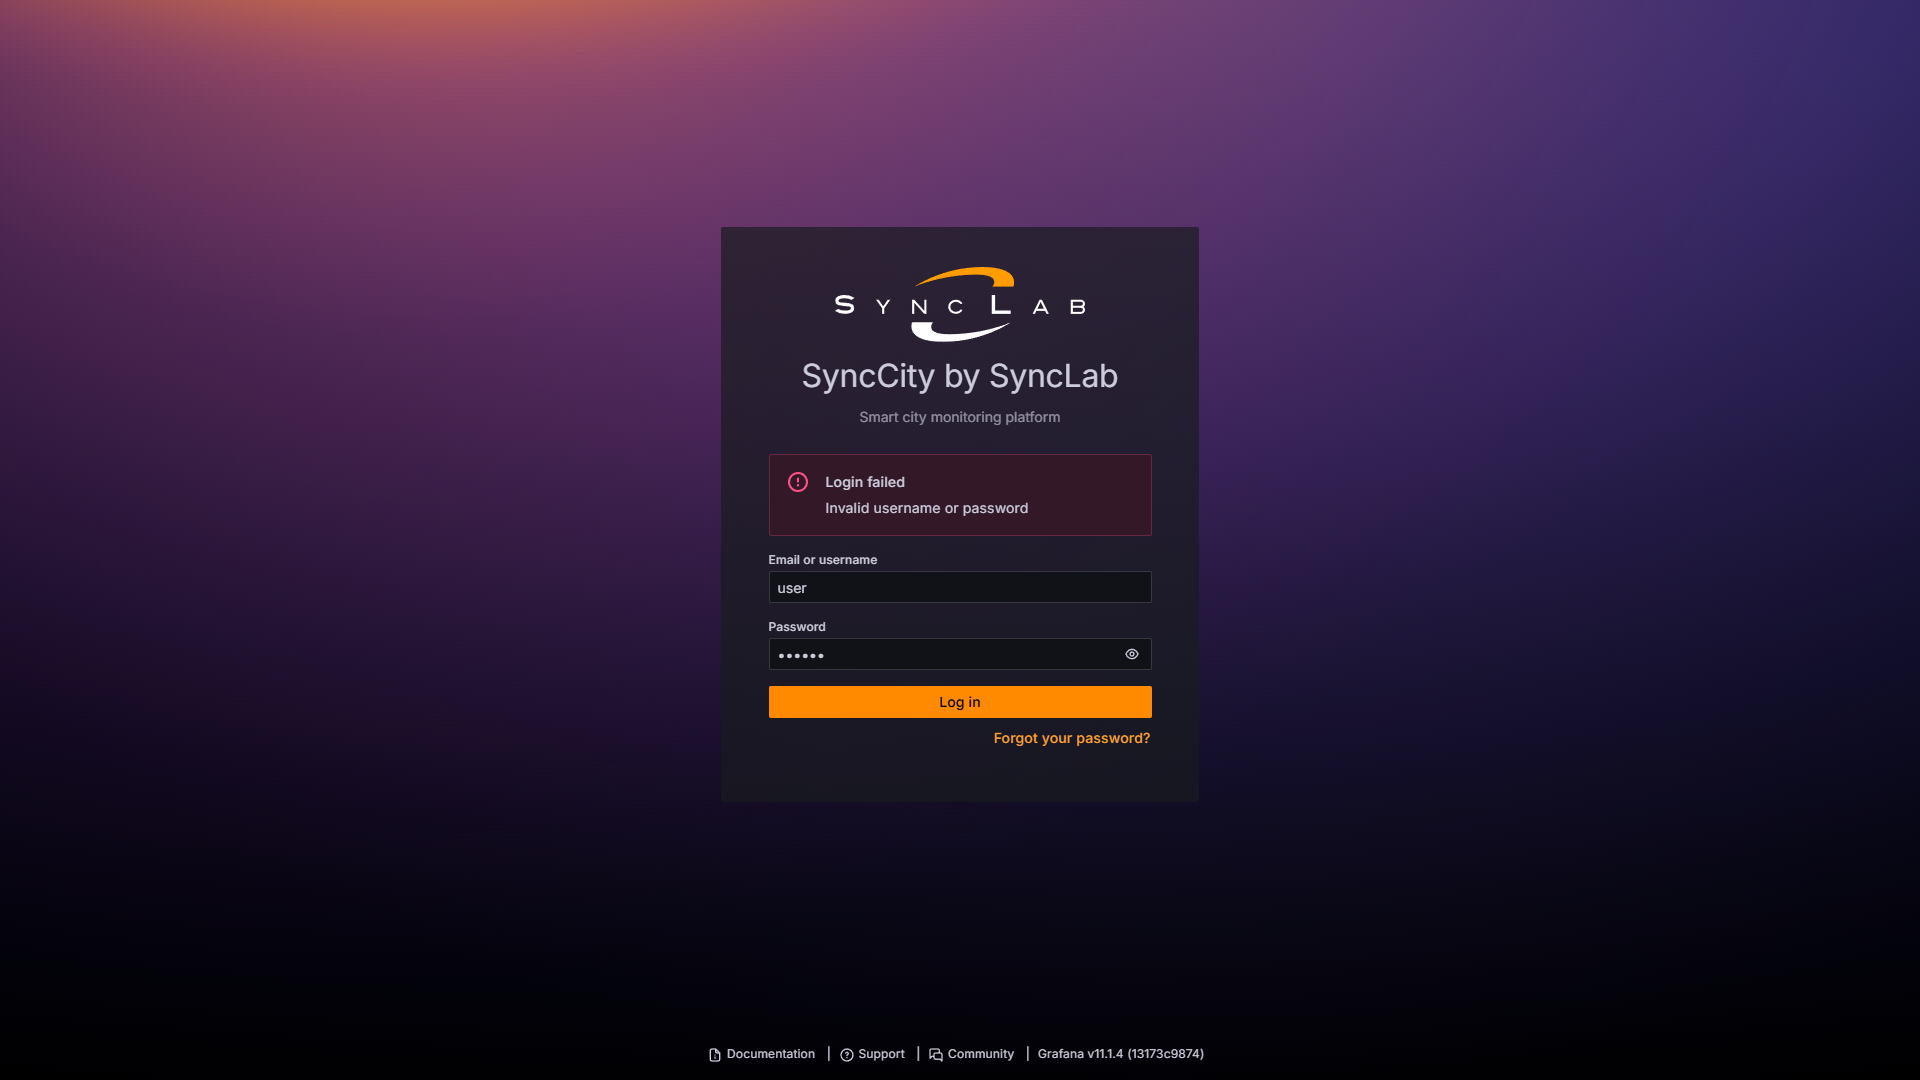
\includegraphics[width=15cm]{./images_mu/login_error.png}
    \caption{Messaggio di errore inserimento credenziali errate.}
    \label{figure:Messaggio di errore inserimento credenziali errate.}
\end{figure}
\subsection{Home}
Una volta effettuato l'accesso, l'utente viene indirizzato alla pagina ``\glossterm{Dashboards}". 
In questa schermata è possibile visualizzare tutte le dashboard che l'applicativo espone, elencate in ordine alfabetico. L'utente può dunque selezionarne una e verrà indirizzato ad una nuova pagina dove potrà visualizzare tutti i pannelli contenuti nel cruscotto di proprio interesse.
\begin{figure}[H]
    \centering
    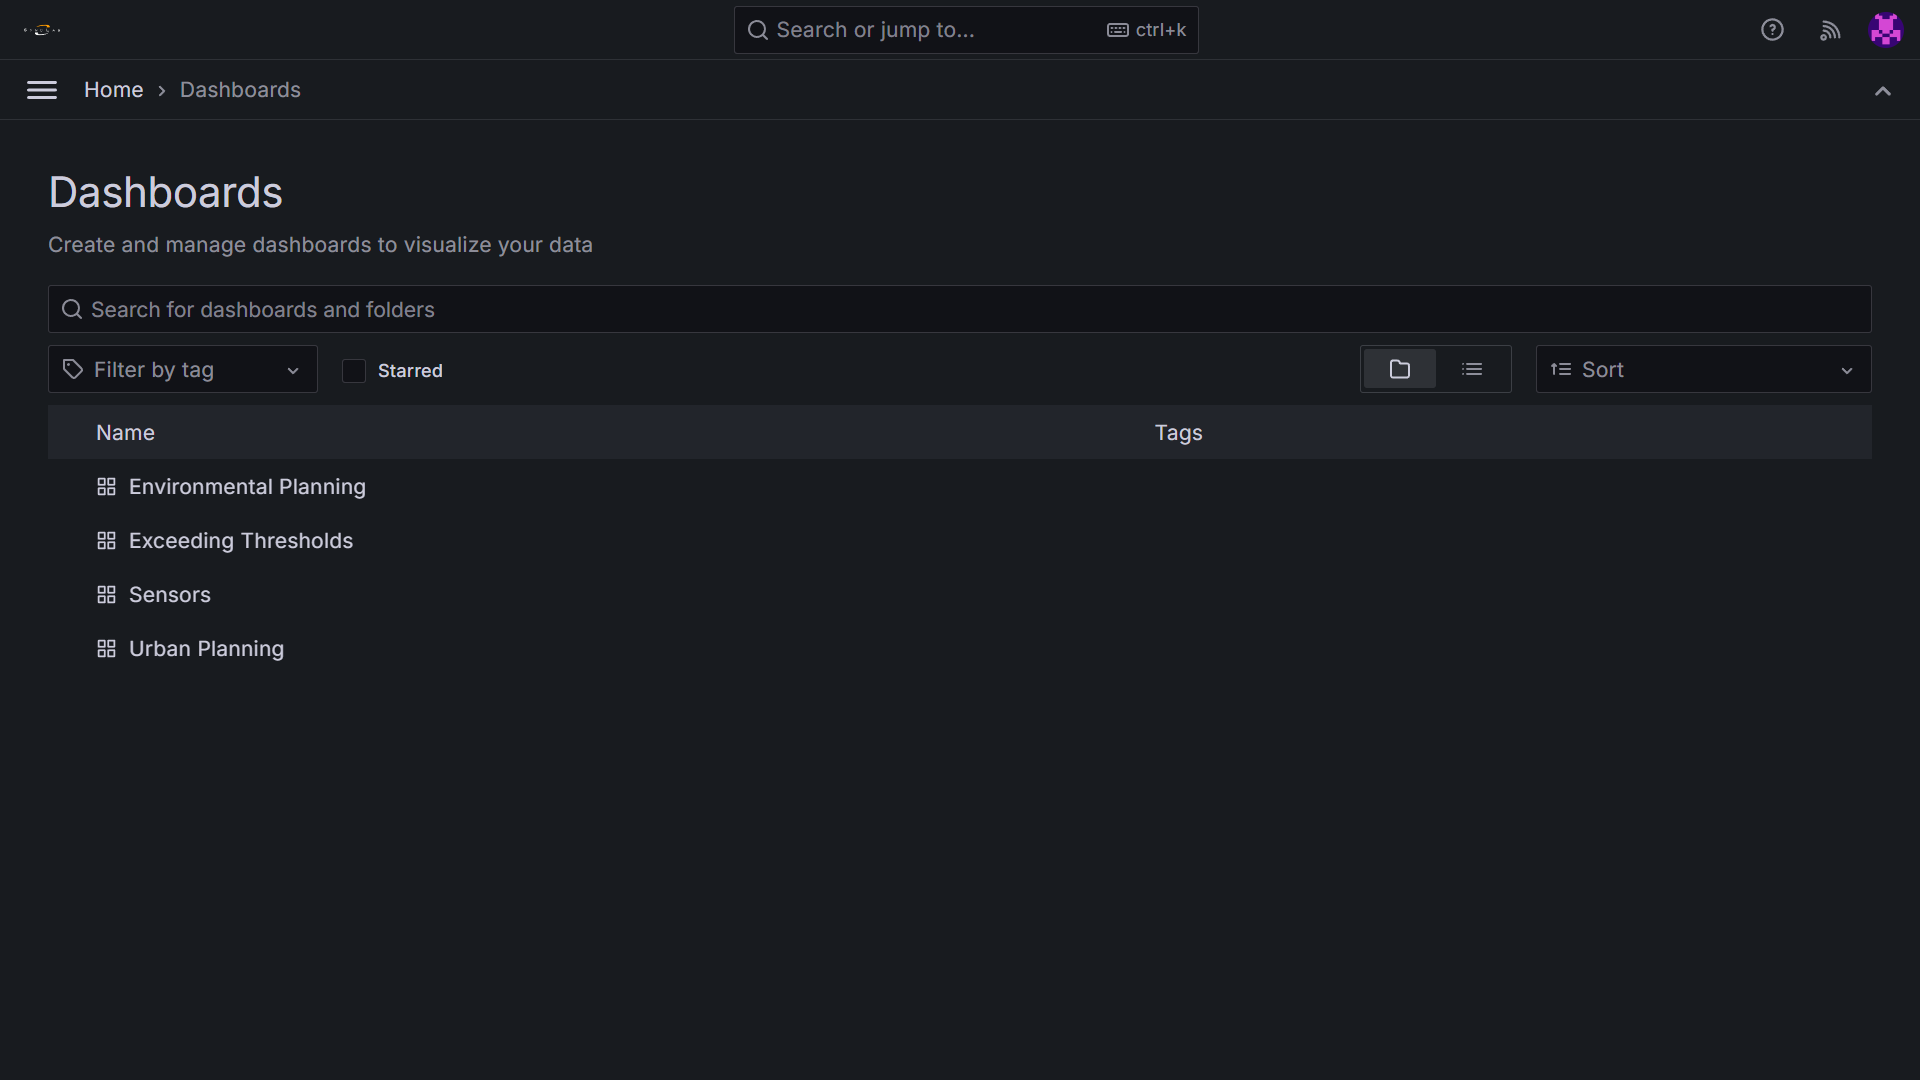
\includegraphics[width=15cm]{./images_mu/dashboards.png}
    \caption{Schermata ``Dashboards".}
    \label{figure:Schermata Dashboards.}
\end{figure}
Oltre all'elenco delle dashboard, in questa pagina si trovano altri elementi utili all'utente che ricorreranno in tutte le schermate dell'applicativo, descritti alle sezioni seguenti.

\subsubsection{Barra di ricerca} 
Permette di cercare dashboard, pagine dell'applicativo, azioni e impostazioni digitandone il nome. Cliccando su uno dei risultati di ricerca, l'utente viene indirizzato alla schermata selezionata.
\begin{figure}[H]
    \centering
    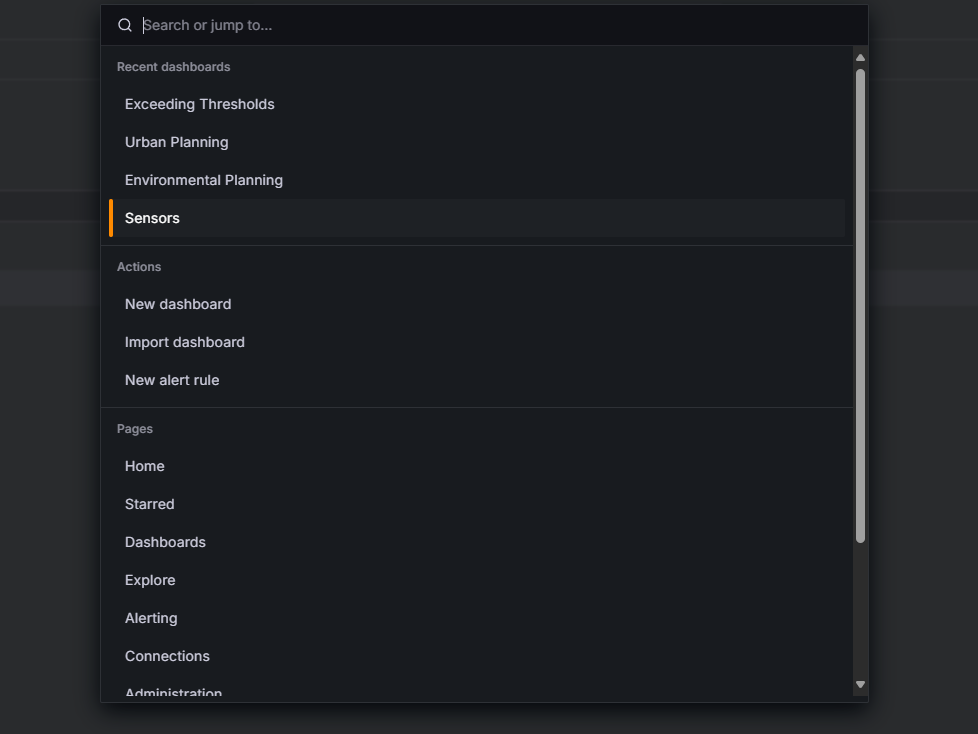
\includegraphics[width=8cm]{./images_mu/search.png}
    \caption{Barra di ricerca.}
    \label{figure:Barra di ricerca.}
\end{figure}

\subsubsection{Pulsante profilo utente}
Cliccando sull'icona contenente l'immagine profilo dell'utente è possibile visualizzare un menu a tendina con le seguenti opzioni:
\begin{itemize}
    \item \textbf{Profile:} apre una pagina grazie alla quale è possibile visualizzare e modificare le proprie informazioni personali (nome, indirizzo email e username) e preferenze dell'applicativo (tema chiaro o scuro, dashboard di default, fuso orario, giorno di inizio della settimana e lingua);
    \item \textbf{Notification history:} consente di visualizzare la cronologia delle notifiche ricevute;
    \item \textbf{Change password:} permette di reimpostare la password dell'account;
    \item \textbf{Sign out:} effettua la disconnessione dell'utente, reindirizzando alla pagina di login.
\end{itemize}
\begin{figure}[H]
    \centering
    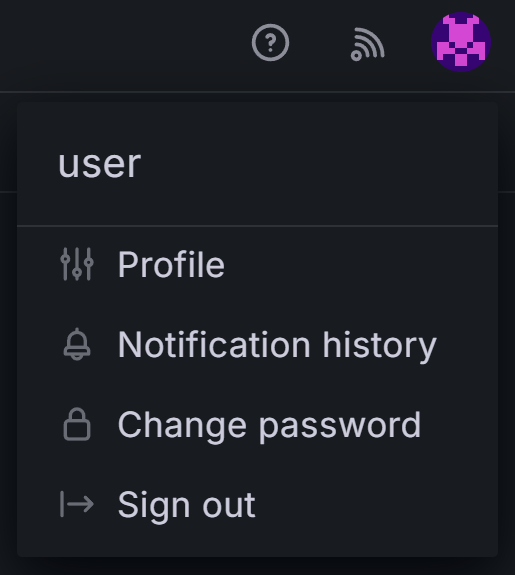
\includegraphics[width=7cm]{images_mu/profile.png}
    \caption{Pulsante profilo utente.}
    \label{fig:Pulsante profilo utente}
\end{figure}

\subsubsection{Barra degli strumenti} 
Contiene diverse funzionalità che agevolano l'utente nella fruizione dell'applicativo e garantiscono un'esperienza di utilizzo completa. Di seguito sono elencate tutte le icone presenti e il relativo scopo:
\begin{itemize}
    \item \textbf{Menu ad hamburger:} contraddistinto dalla caratteristica icona con le tre linee orizzontali sovrapposte, si tratta di un menu a comparsa che semplifica la navigazione tra le diverse pagine. Infatti, ciascun elemento del menu rimanda ad una schermata dell'applicazione a cui l'utente può facilmente accedere. Tra esse, ne citiamo alcune: 
    \begin{itemize}
        \item Starred: consente di vedere le dashboard che l'utente ha aggiunto tra le preferite;
        \item Alerting: permette di visualizzare le informazioni relative alle notifiche inviate dal sistema.
    \end{itemize}
    \begin{figure}[H]
        \centering
        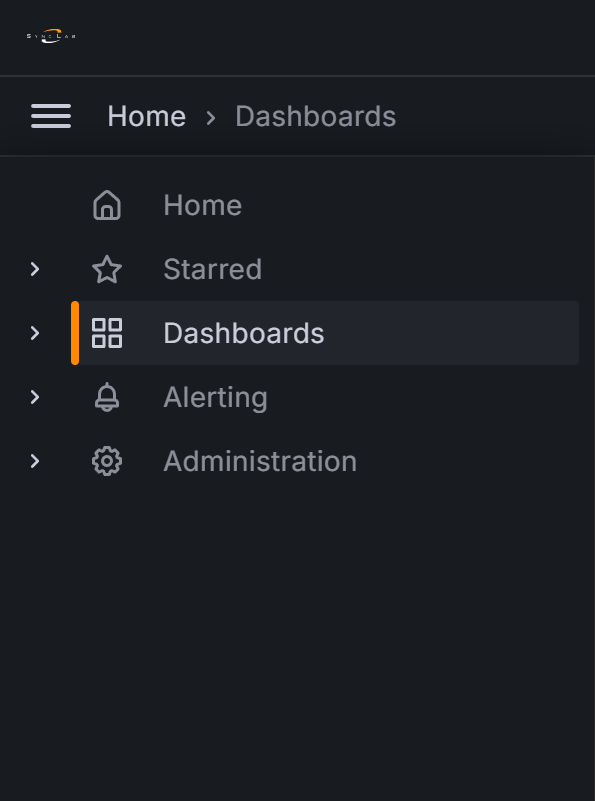
\includegraphics[width=7cm]{./images_mu/hamburger_menu.png}
        \caption{Menu ad hamburger.}
        \label{figure:Menu ad hamburger.}
    \end{figure}
    \item \textbf{Breadcrumb:} segnala la posizione attuale dell'utente all'interno dell'applicativo;
    \begin{figure}[H]
        \centering
        
\includegraphics[width=9cm]{./images_mu/breadcrumb.png}
        \caption{Breadcrumb.}
        \label{figure:Breadcrumb.}
    \end{figure}
    \item \textbf{Aggiungi ai preferiti:} questo pulsante serve per contrassegnare una dashboard come preferita. Essa comparirà quindi nella sezione ``Starred".
    \begin{figure}[H]
        \centering
        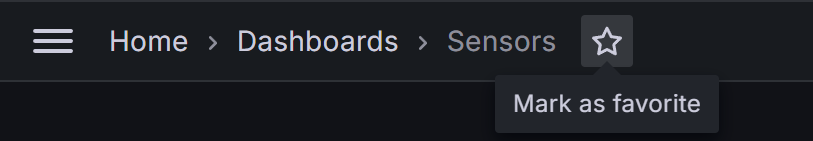
\includegraphics[width=10cm]{images_mu/star.png}
        \caption{Pulsante ``Aggiungi ai preferiti".}
        \label{fig:Pulsante ``Aggiungi ai preferiti"}
    \end{figure}
\end{itemize}
\subsection{Informazioni generali dashboard e pannelli}
Una dashboard consiste in un cruscotto che racchiude al suo interno diversi \glossterm{widget}, cioè pannelli. Ciascuno di essi permette di visualizzare i dati in tempo reale provenienti dai sensori oppure informazioni aggiuntive, ricavate aggregando ed elaborando le suddette misurazioni. 
\subsubsection{Strumenti dashboard}
Una volta che l'utente avrà selezionato un cruscotto da visualizzare, nella barra degli strumenti saranno disponibili altre opzioni specifiche per le dashboard:
\begin{itemize}
    \item \textbf{Intervallo temporale:} questo menu a tendina consente di selezionare l'intervallo temporale di visualizzazione dei dati. È possibile scegliere tra diverse opzioni predefinite ma anche definire un intervallo personalizzato. Una volta selezionato l'intervallo desiderato, tutti i pannelli presenti all'interno della dashboard aggiorneranno di conseguenza i dati mostrati;
    \begin{figure}[H]
        \centering
        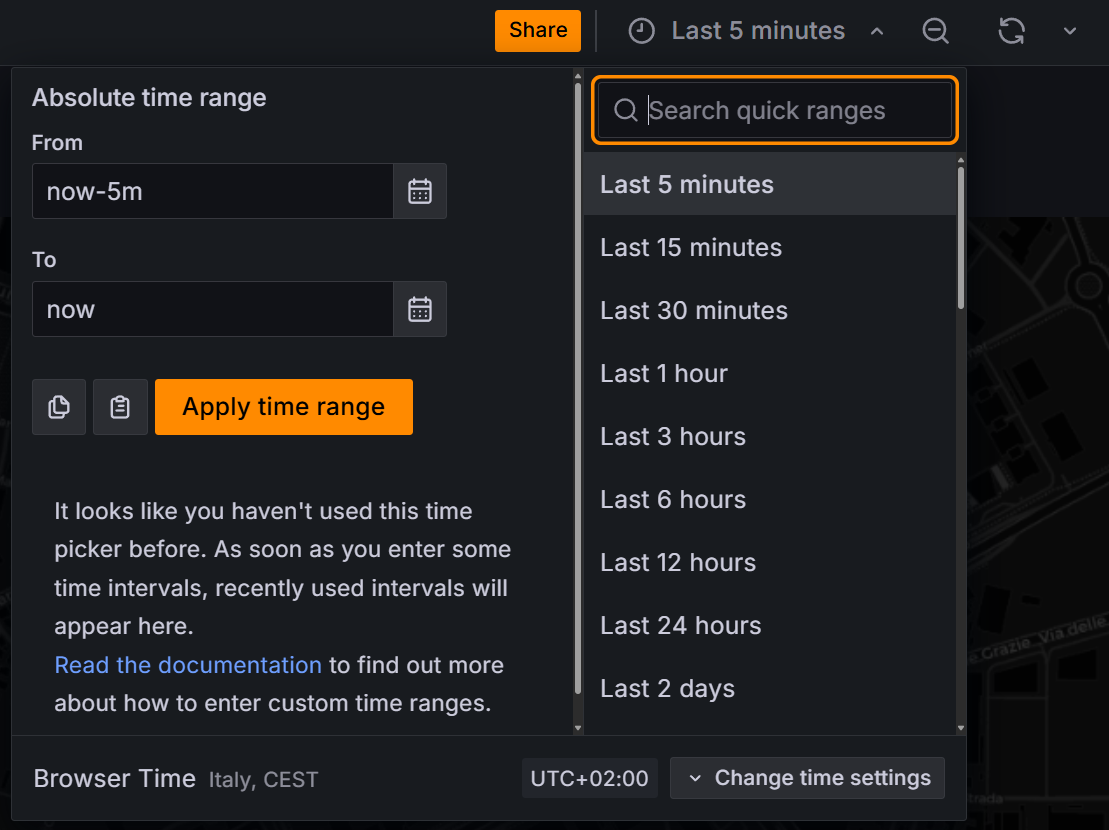
\includegraphics[width=10cm]{images_mu/interval.png}
        \caption{Menu di selezione dell'intervallo temporale.}
        \label{fig:Menu di selezione dell'intervallo temporale"}
    \end{figure}
    \item \textbf{Zoom out:} questo pulsante permette di ampliare l'intervallo temporale di visualizzazione dei dati secondo intervalli predefiniti;
    \begin{figure}[H]
        \centering
        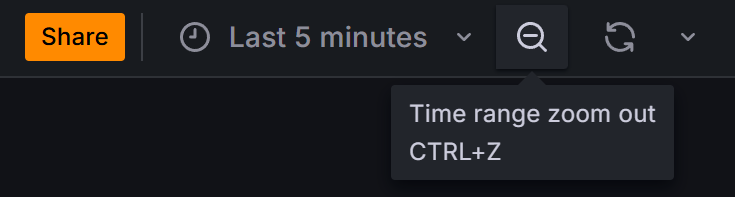
\includegraphics[width=10cm]{images_mu/zoom.png}
        \caption{Pulsante ``Zoom out".}
        \label{fig:Pulsante ``Zoom out"}
    \end{figure}
    \item \textbf{Ricarica dashboard:} questo pulsante aggiorna la dashboard in modo da mostrare i dati più recenti. È possibile ricaricare la dashboard cliccando sul pulsante oppure attivare il refresh automatico, selezionando una tra le frequenze di aggiornamento disponibili nell'apposito menu a tendina.
    \begin{figure}[H]
        \centering
        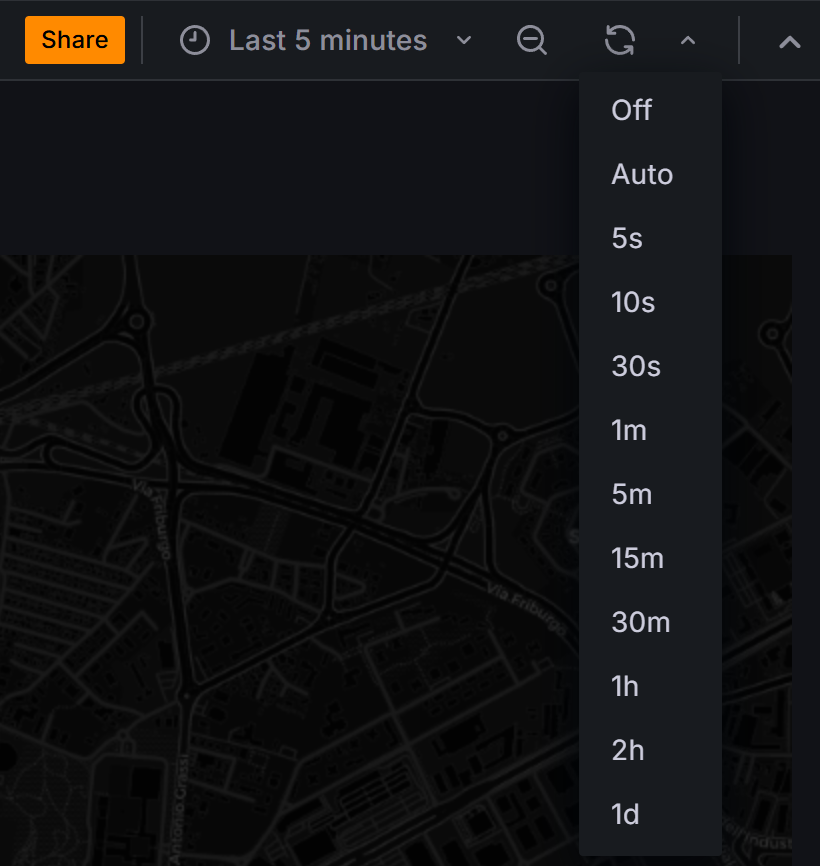
\includegraphics[width=10cm]{images_mu/refresh.png}
        \caption{Pulsante ``Ricarica dashboard".}
        \label{fig:Pulsante ``Ricarica dashboard"}
    \end{figure}
\end{itemize}
\subsubsection{Selezione variabili}
Per ciascuna tipologia di sensore è possibile visualizzare contemporaneamente i dati provenienti da uno o più rilevatori. Le dashboard che contengono pannelli relativi a tipi di dati differenti offrono quindi la possibilità di selezionare, grazie ad appositi menu a tendina, i singoli dispositivi di cui si vogliono osservare le misurazioni, aggiornando di conseguenza tutti i pannelli coinvolti dalla selezione. 
\begin{figure}[H]
        \centering
        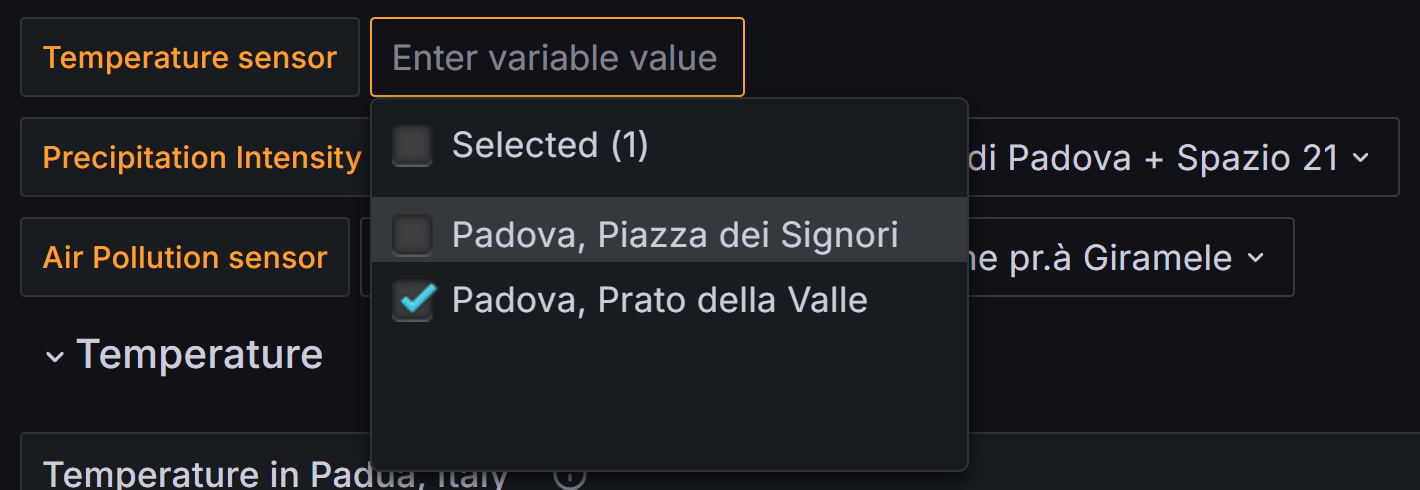
\includegraphics[width=10cm]{images_mu/environmental_variables.png}
        \caption{Variabili dashboard ``Ambientale" con menu di selezione.}
        \label{fig:Variabili dashboard Ambientale con menu di selezione"}
    \end{figure}
    \begin{figure}[H]
        \centering
        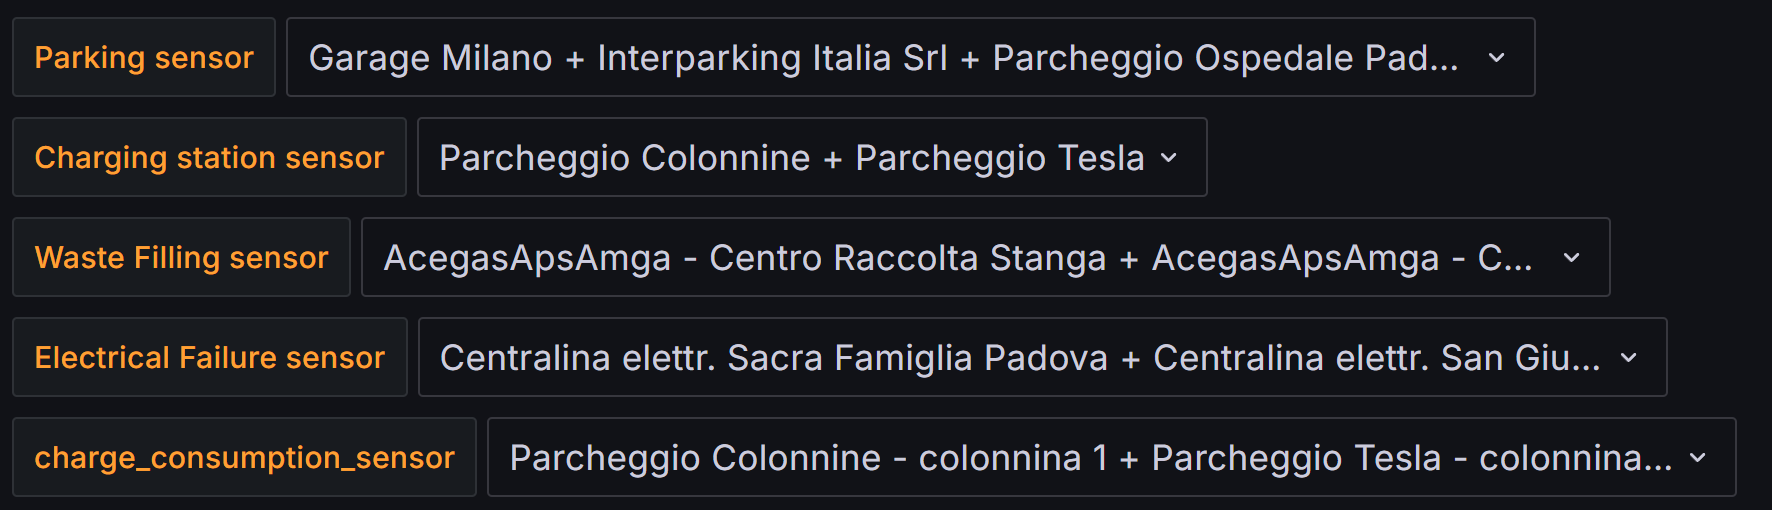
\includegraphics[width=10cm]{images_mu/urban_variables.png}
        \caption{Variabili dashboard ``Urbanistica".}
        \label{fig:Variabili dashboard urbanistica"}
    \end{figure}
\subsubsection{Righe}
Una riga consiste in un raggruppamento di pannelli. Il suo funzionamento è simile a quello di un menu a tendina, infatti l'utente può visualizzare o nascondere i widget contenuti al suo interno cliccando sul nome della riga. All'interno delle varie dashboard, i pannelli sono suddivisi a seconda della tipologia di dato mostrato. 
\begin{figure}[H]
    \centering
    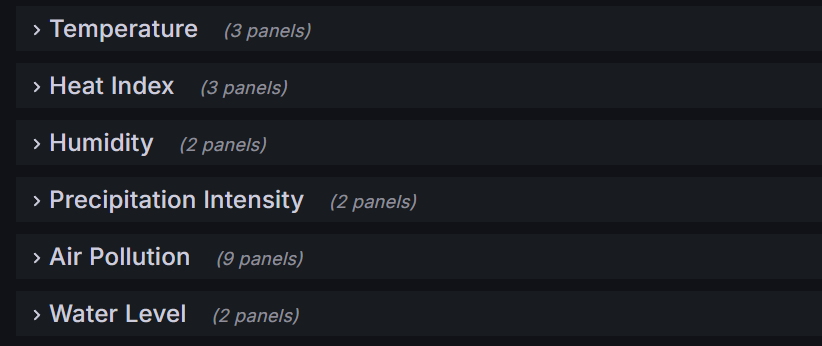
\includegraphics[width=10cm]{images_mu/rows.png}
    \caption{Esempio di suddivisione dei pannelli in righe: ``dashboard Ambientale".}
    \label{fig:Esempio di suddivisione dei pannelli in righe: ``dashboard Ambientale"}
\end{figure}
\subsubsection{Pannelli}
Un pannello, anche chiamato widget, consiste in un grafico adibito alla visualizzazione di un determinato tipo di dato. Ogni dashboard può contenere da uno a molteplici widget, ciascuno dei quali espone:
\begin{itemize}
\setlength\itemsep{0em}
    \item Il nome del pannello, che coincide con la tipologia di dato raffigurato;
    \item Una breve descrizione, esplicativa del contenuto del widget;
    \item Se è possibile ricevere delle notifiche riguardanti il tipo di dato visualizzato dal pannello, è presente anche un'icona che indica se le misurazioni attuali stanno facendo scattare un'allerta (per maggiori dettagli sulle notifiche si rimanda alla sezione \ref{sec:alert});
    \item La legenda del grafico, per facilitare la comprensione dei dati;
    \item Un menu a tendina contenente diverse opzioni, che consentono di visualizzare il singolo pannello occupando l'intera finestra, condividere il pannello, ispezionare le misurazioni mostrate e la configurazione del pannello e infine nascondere o mostrare la legenda.
    \item Il grafico vero e proprio, contenente le rilevazioni effettuate in tempo reale o informazioni aggiuntive ricavate dalle misurazioni stesse.
\end{itemize}
I pannelli possono essere di diversi formati e dimensioni, in modo da trasmettere l'informazione d'interesse in maniera efficace e comprensibile all'utente. Di seguito sono descritte tutte le tipologie di pannelli presenti all'interno dell'applicativo.

\subsubsubsection{\glossterm{Geomap}}
I widget in formato ``Geomap" consistono in mappe interattive che segnalano la posizione di un elemento di interesse, quale può essere ad esempio un sensore, all'interno dell'area geografica visualizzata. È possibile visualizzare diverse aree della mappa tenendo premuto e trascinando il cursore, oltre a effettuare lo zoom grazie agli appositi pulsanti ``+" e ``-". 
\subsubsubsection{\glossterm{Time series}}
I widget in formato ``Time series" consistono in grafici cartesiani che descrivono l'andamento nel tempo delle misurazioni effettuate dai sensori. In particolare, l'asse x riporta il momento in cui viene effettuata una rilevazione mentre sull'asse y vi sono i valori misurati. Ciascuna linea del grafico rappresenta un singolo sensore e posizionando il cursore su di essa è possibile vedere l'ora precisa del rilevamento e il valore esatto misurato. L'utente può inoltre restringere l'intervallo temporale mostrato dal singolo pannello selezionando la porzione di linea che si desidera visualizzare nel dettaglio.

\subsubsubsection{\glossterm{Gauge}}
I widget in formato ``Gauge" visualizzano un singolo valore numerico calcolato sulla base di una serie di misurazioni. Il pannello ricorda graficamente un manometro e il valore mostrato cambia colore a seconda che esso superi o meno le soglie impostate. Questo tipo di widget non è interattivo.

\subsubsubsection{\glossterm{Bar chart}}
I widget in formato ``Bar chart" consistono in istogrammi che consentono all'utente di visualizzare in maniera immediata il confronto tra più dati categorici. In particolare, nell'applicativo vengono utilizzati per esprimere il paragone tra le rilevazioni minime e massime registrate, oltre che tra valori calcolati sulla base delle misurazioni come media aritmetica e moda. L'utente può posizionare il cursore sopra le colonne del grafico per visualizzarne i dettagli, quali nome del sensore coinvolto, categoria del dato e valore esatto.

\subsubsubsection{Table}
I widget in formato ``Table" consistono in tabelle le cui righe vengono aggiornate automaticamente ad ogni misurazione. Questo tipo di pannello consente all'utente di cogliere tutti i dettagli delle rilevazioni effettuate, specialmente nei casi in cui i dati inviati dai sensori non includono soltanto un unico valore numerico ma molteplici informazioni. L'utente può interagire con la tabella cliccando sull'intestazione di una colonna, in modo da ordinare i dati alfabeticamente secondo il valore contenuto in quel tipo di cella.

\subsubsubsection{Log}
I widget in formato ``Log" consistono in elenchi testuali di informazioni provenienti dal database. Nell'applicativo sono utilizzati unicamente per registrare i pagamenti avvenuti. L'utente può interagire con il pannello cliccando su una riga dell'elenco, visualizzando ulteriori dettagli.

\subsubsubsection{Bar gauge}
I widget in formato ``Bar gauge" sono molto simili graficamente e nella loro funzione ai pannelli in formato ``Bar chart". Infatti, si tratta di ortogrammi a nastro che consentono di confrontare tra loro rilevazioni massime, minime e medie. La differenza con gli istogrammi risiede nell'orientamento delle barre dei dati, che in questo caso sono orizzontali e non colonnari, e nel fatto che affianco ad ogni nastro è indicato anche il valore numerico corrispondente. L'utente non deve quindi posizionare il cursore sopra al grafico per ottenere maggiori informazioni, poiché tutte quelle disponibili sono già visibili. Esattamente come i pannelli di tipo ``Gauge", questo tipo di widget non è interattivo.

\subsubsubsection{Alert list}
I widget in formato ``Alert list" consistono in una lista di notifiche, dove ciascun elemento dell'elenco è corredato di nome (che coincide con il tipo di dato monitorato), stato e istanze dell'allerta. Nel caso in cui sia scattata l'allerta è possibile vedere da quanto tempo i valori misurati sono fuori norma. È disponibile anche un menu a tendina che permette di visualizzare i dettagli di ciascuna notifica.

\subsection{Dashboard ``Sensori"}
La dashboard ``Sensors" ospita al suo interno un unico pannello, ovvero una mappa che indica la posizione di ciascun sensore presente all'interno del territorio urbano. I sensori sono raffigurati mediante icone differenti a seconda della tipologia di dato rilevato. L'utente può dedurre l'icona corrispondente a ciascun tipo di sensore grazie alla legenda. Posizionando il cursore sopra un'icona o semplicemente cliccandola, è possibile visualizzare le informazioni relative al sensore selezionato, quali tipologia, nome e coordinate geografiche. È possibile effettuare lo zoom sulla mappa per visualizzare la posizione esatta di un sensore o per avere una visione panoramica di tutti i rilevatori disponibili.
\begin{figure}[H]
    \centering
    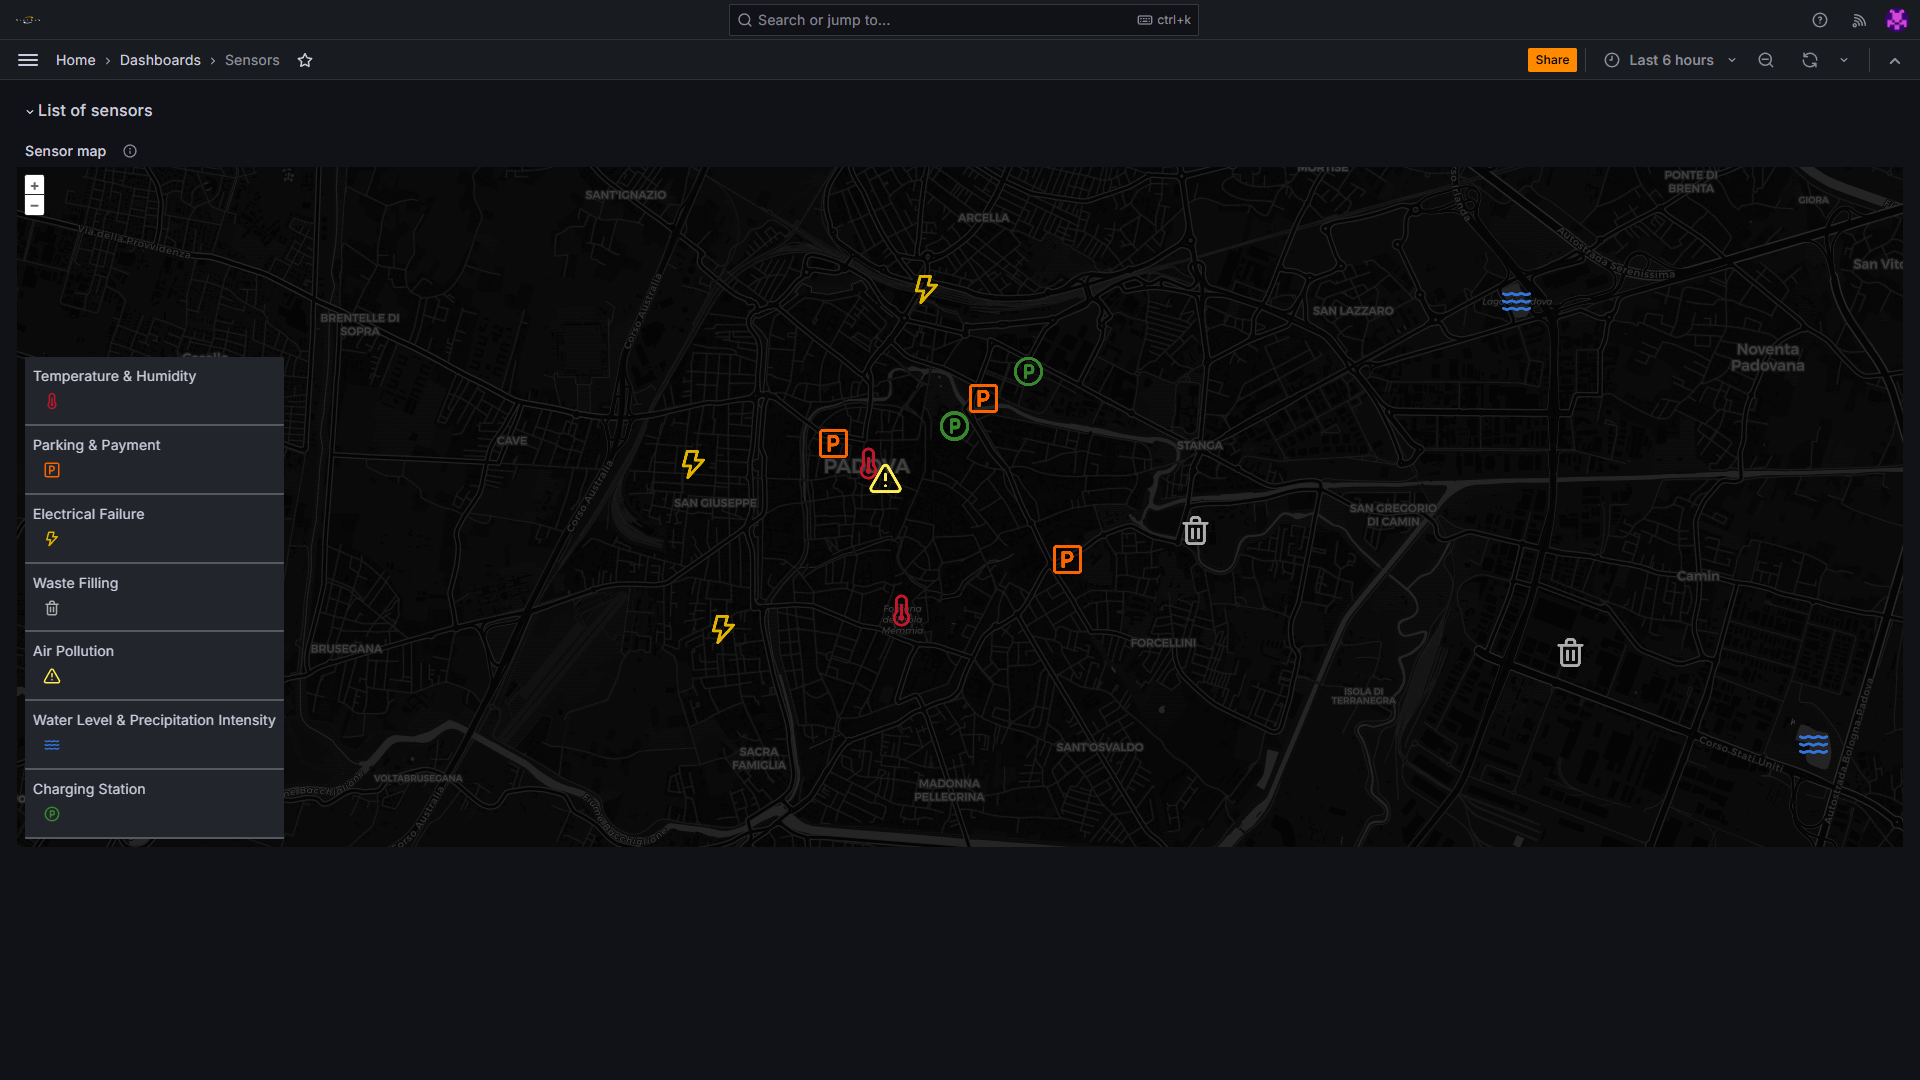
\includegraphics[width=15cm]{images_mu/sensors.png}
    \caption{Dashboard ``Sensori".}
    \label{fig:Dashboard ``Sensori"}
\end{figure}
\subsection{Dashboard ``Ambientale"}
La dashboard ``Environmental Planning" consente di visualizzare i dati relativi all'ambiente, ovvero temperatura (effettiva e percepita), umidità, intensità delle precipitazioni, inquinamento atmosferico e livello di riempimento dei bacini idrici. La dashboard è suddivisa in sei righe, una per ogni tipologia di dato, contenenti uno o più pannelli. Alle sezioni seguenti viene illustrato il contenuto di ciascuna riga.
\subsubsection{Temperatura}
\begin{itemize}
\setlength\itemsep{0em}
    \item Pannello time series che mostra l'andamento delle rilevazioni nel tempo;
    \item Istogramma che visualizza, per ciascun sensore disponibile, rilevazione minima e massima, media aritmetica e moda;
    \item Pannello Gauge che mostra il valore esatto della temperatura media, combinando le misurazioni di tutti i sensori di temperatura presenti in città.
\end{itemize}
\begin{figure}[H]
    \centering
    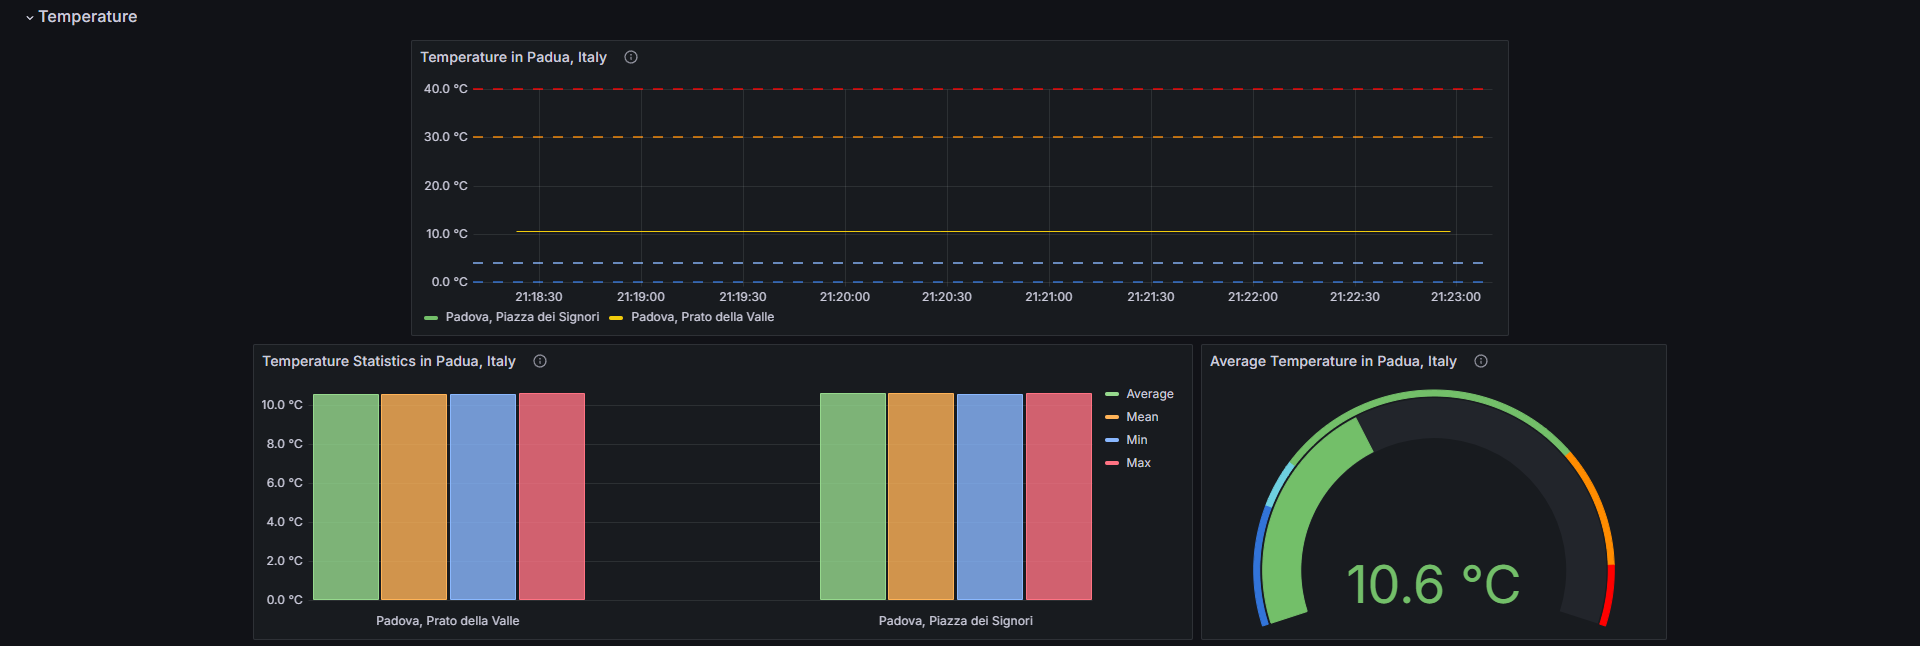
\includegraphics[width=15cm]{images_mu/temperature.png}
    \caption{Pannelli relativi alla temperatura.}
    \label{fig:Pannelli relativi alla temperatura}
\end{figure}
\subsubsection{Temperatura percepita}
\begin{itemize}
\setlength\itemsep{0em}
    \item Pannello time series che mostra l'andamento delle rilevazioni nel tempo;
    \item Istogramma che visualizza, per ciascun sensore disponibile, rilevazione minima e massima e media aritmetica;
    \item Pannello Gauge che mostra il valore esatto della temperatura media percepita, combinando le misurazioni di tutti i sensori di temperatura presenti in città.
\end{itemize}
\begin{figure}[H]
    \centering
    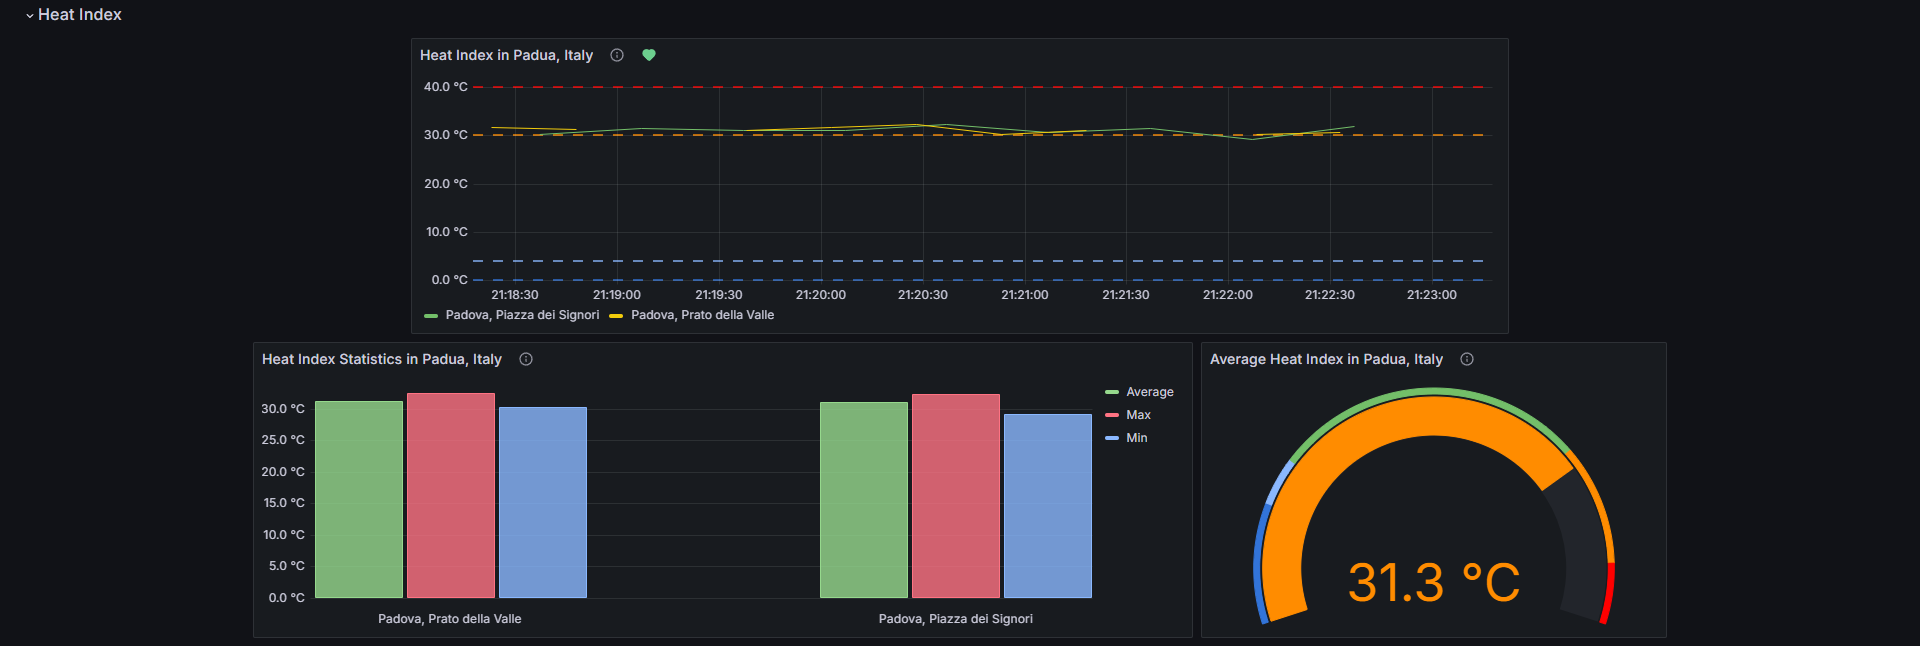
\includegraphics[width=15cm]{images_mu/heat_index.png}
    \caption{Pannelli relativi alla temperatura percepita.}
    \label{fig:Pannelli relativi alla temperatura percepita}
\end{figure}
\subsubsection{Umidità}
\begin{itemize}
\setlength\itemsep{0em}
    \item Pannello time series che mostra l'andamento delle rilevazioni nel tempo;
    \item Pannello Gauge che mostra il valore esatto dell'umidità media, combinando le misurazioni di tutti i sensori di umidità in città.
\end{itemize}
\begin{figure}[H]
    \centering
    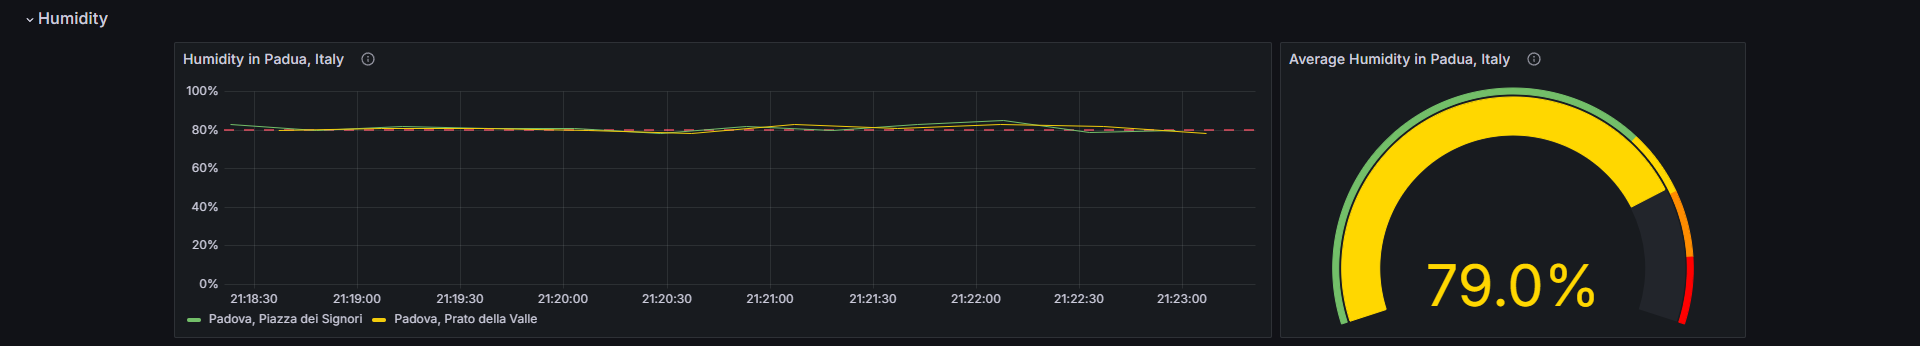
\includegraphics[width=15cm]{images_mu/humidity.png}
    \caption{Pannelli relativi all'umidità.}
    \label{fig:Pannelli relativi all'umidità}
\end{figure}
\subsubsection{Intensità delle precipitazioni}
\begin{itemize}
\setlength\itemsep{0em}
    \item Pannello time series che mostra l'andamento delle rilevazioni nel tempo;
    \item Pannello Gauge che mostra il valore esatto dell'intensità media delle precipitazioni, combinando le misurazioni di tutti i sensori di precipitazioni in città.
\end{itemize}
\begin{figure}[H]
    \centering
    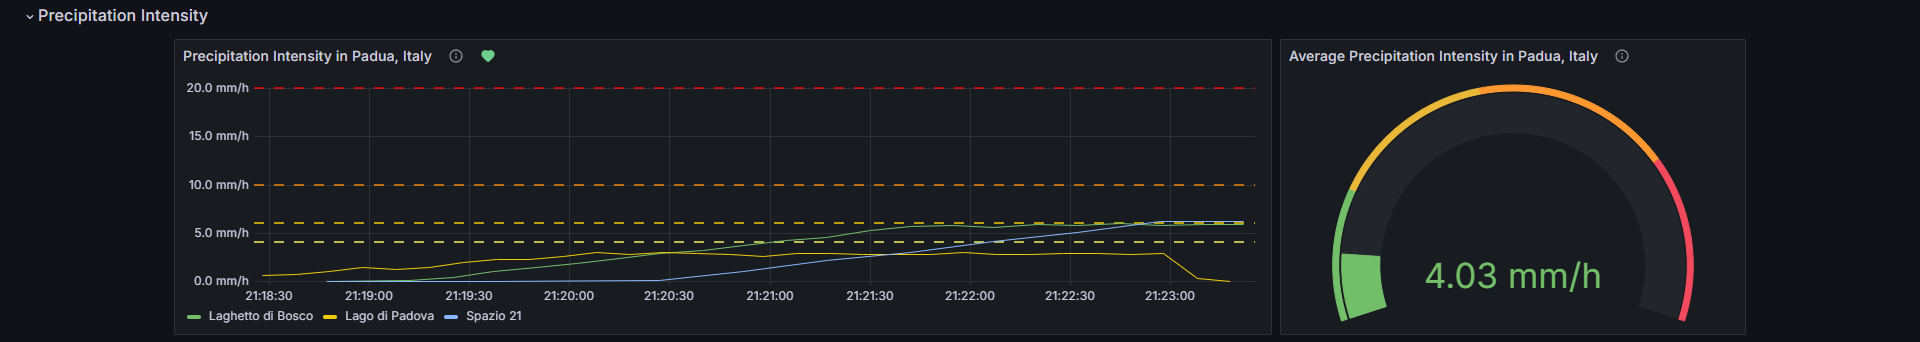
\includegraphics[width=15cm]{images_mu/precipitation_intensity.png}
    \caption{Pannelli relativi all'intensità delle precipitazioni.}
    \label{fig:Pannelli relativi all'intensità delle precipitazioni}
\end{figure}
\subsubsection{Inquinamento dell'aria}
\begin{itemize}
\setlength\itemsep{0em}
    \item Pannello time series che visualizza l'andamento nel tempo dei livelli di inquinamento atmosferico. In questo grafico sono rappresentati tutti i sensori che rilevano il livello di polveri sottili;
    \item Pannello time series che mostra l'andamento nel tempo dei livelli di PM 2.5;
    \item Pannello Gauge che mostra il valore esatto della concentrazione media di PM 2.5;
    \item Pannello time series che mostra l'andamento nel tempo dei livelli di PM 10;
    \item Pannello Gauge che mostra il valore esatto della concentrazione media di PM 10;
    \item Pannello time series che mostra l'andamento nel tempo dei livelli di NO2;
    \item Pannello Gauge che mostra il valore esatto della concentrazione media di NO2;
    \item Pannello time series che mostra l'andamento nel tempo dei livelli di PM O3;
    \item Pannello Gauge che mostra il valore esatto della concentrazione media di O3;
\end{itemize}
\begin{figure}[H]
    \centering
    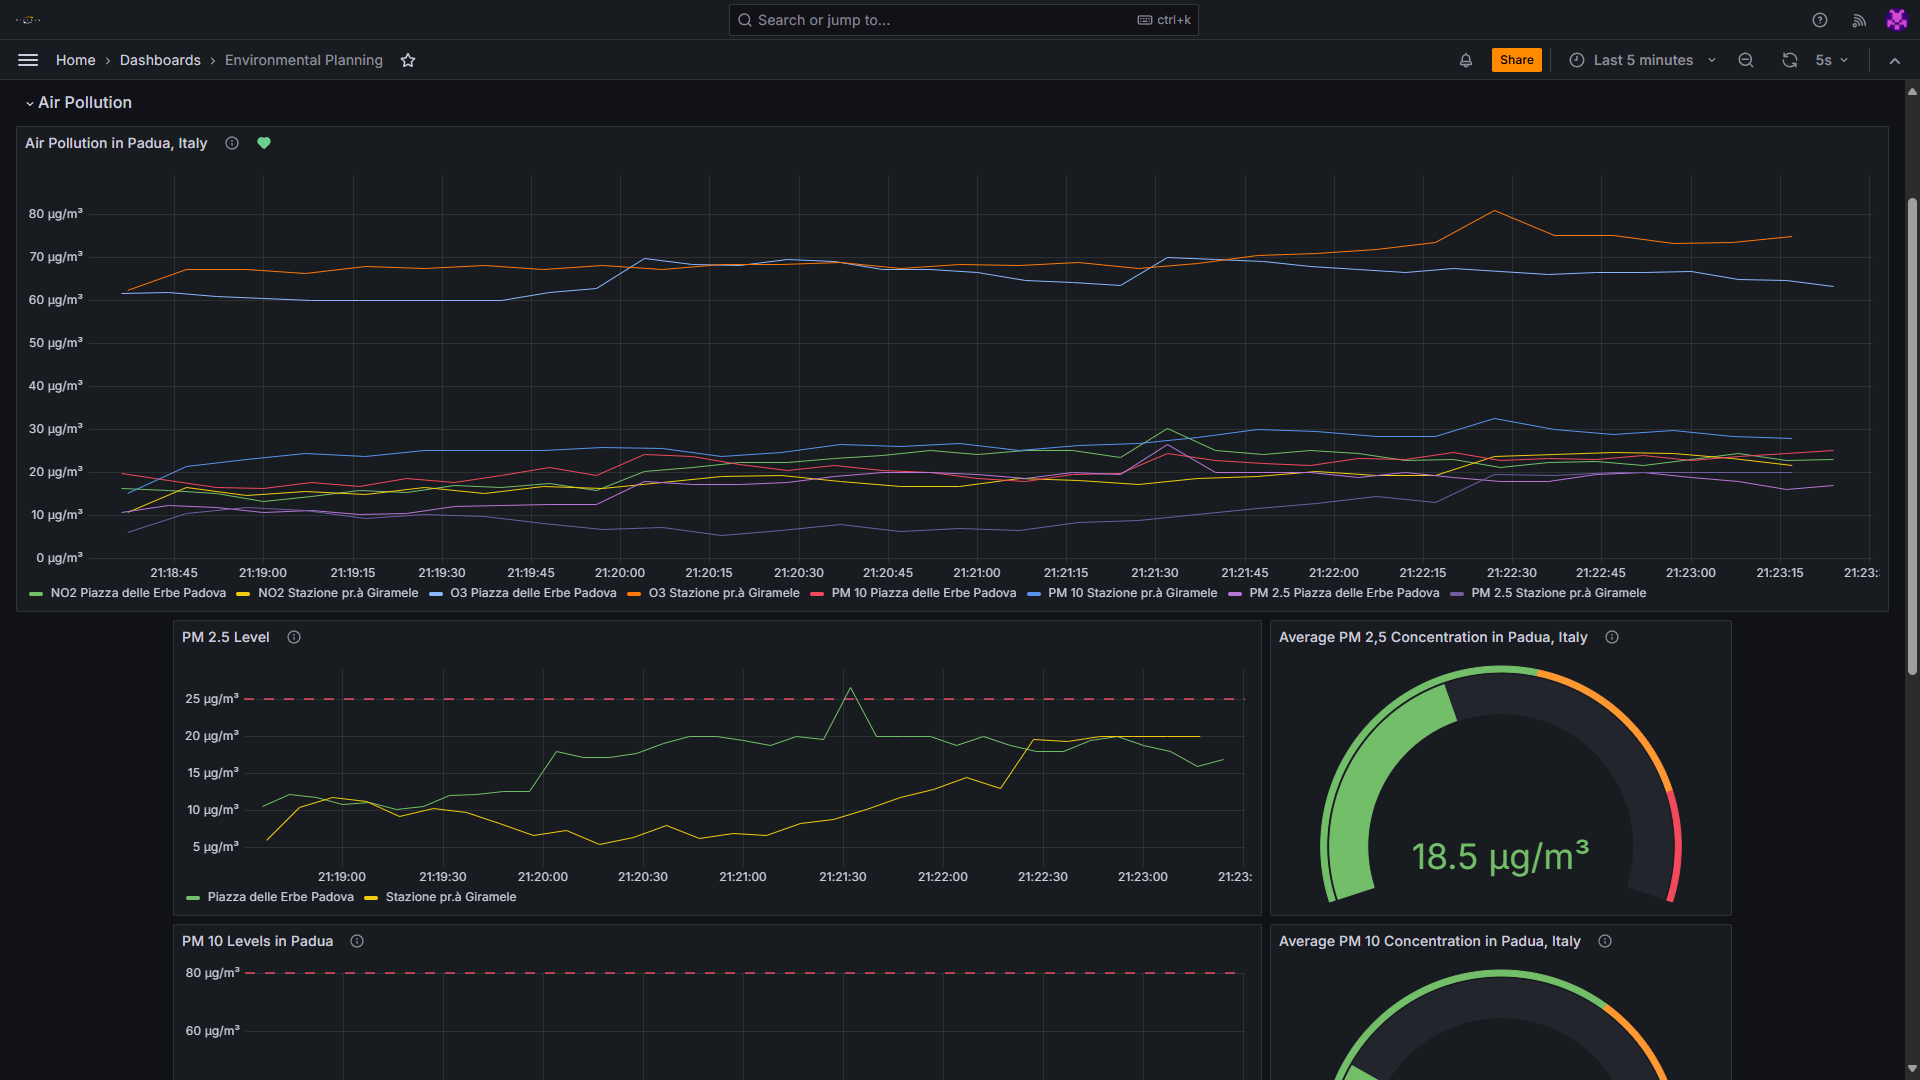
\includegraphics[width=15cm]{images_mu/air_pollution1.png}
    \caption{Prima parte pannelli relativi all'inquinamento atmosferico.}
    \label{fig:Prima parte pannelli relativi all'inquinamento atmosferico}
\end{figure}
\begin{figure}[H]
    \centering
    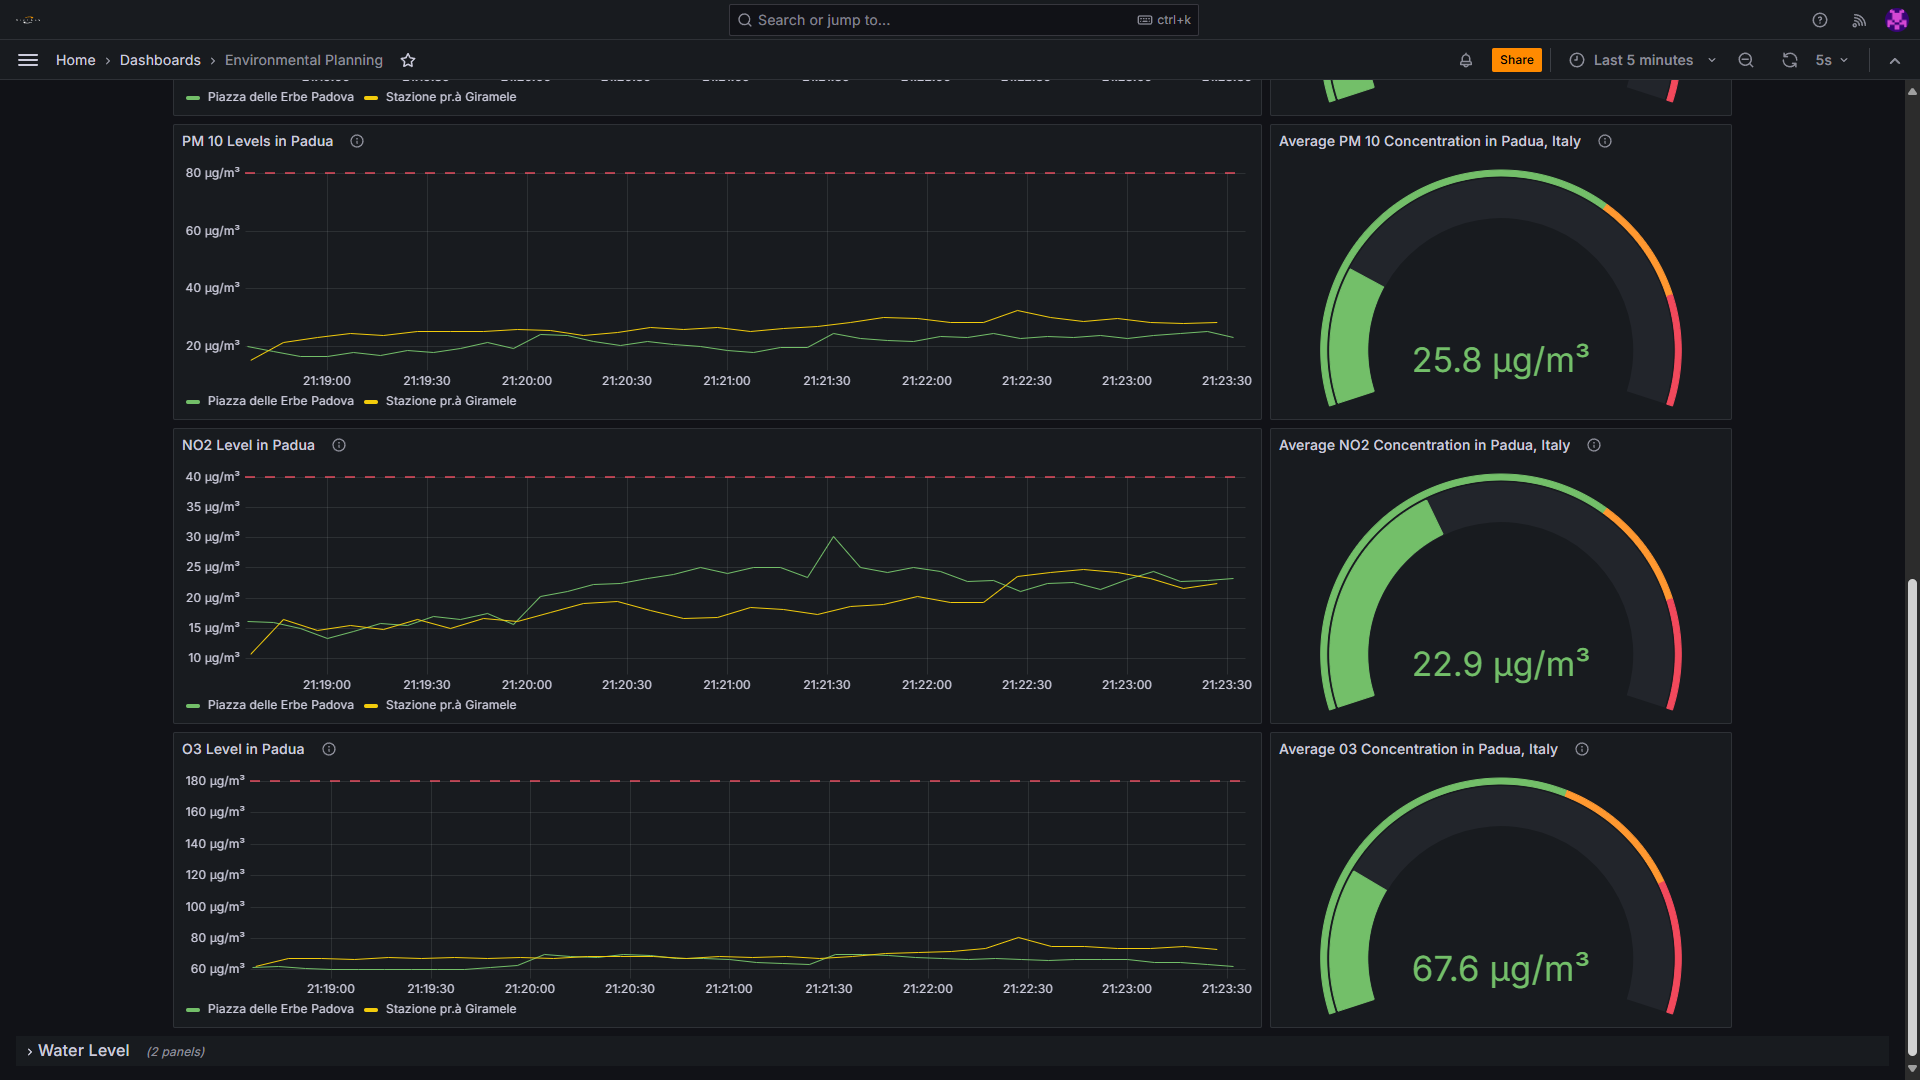
\includegraphics[width=15cm]{images_mu/air_pollution2.png}
    \caption{Seconda parte pannelli relativi all'inquinamento atmosferico.}
    \label{fig:Seconda parte pannelli relativi all'inquinamento atmosferico}
\end{figure}
\subsubsection{Livello dell'acqua}
\begin{itemize}
\setlength\itemsep{0em}
    \item Pannello time series che mostra l'andamento delle rilevazioni nel tempo;
    \item Pannello Gauge che mostra il valore esatto del livello medio di riempimento dei bacini idrici, combinando le misurazioni di tutti i sensori che rilevano il livello dell'acqua in città.
\end{itemize}
\begin{figure}[H]
    \centering
    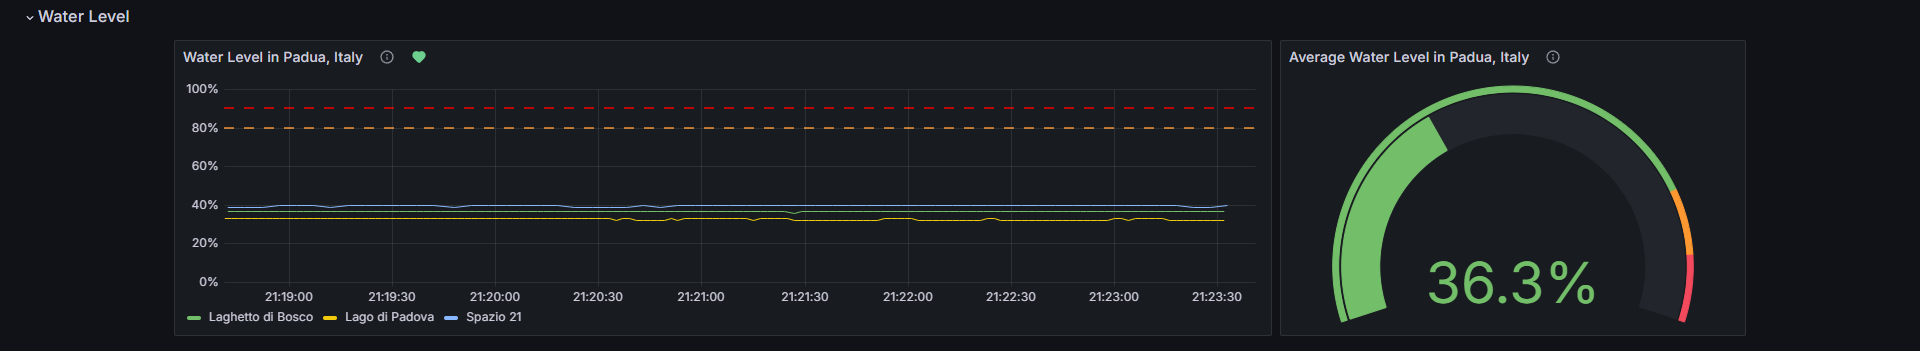
\includegraphics[width=15cm]{images_mu/water_level.png}
    \caption{Pannelli relativi al livello di riempimento dei bacini idrici.}
    \label{fig:Pannelli relativi al livello di riempimento dei bacini idrici.}
\end{figure}
\subsection{Dashboard ``Urbanistica"}
La dashboard ``Urban Planning" consente di visualizzare i dati relativi ai servizi urbani, ovvero parcheggi, colonnine di ricarica per veicoli elettrici, livello di riempimento dei conferitori nelle isole ecologiche e guasti alle centraline elettriche. La dashboard è suddivisa in quattro righe, una per ogni tipologia di dato, contenenti da uno a più pannelli. Alle sezioni seguenti viene illustrato il contenuto di ciascuna riga.
\subsubsection{Parcheggi}
\begin{itemize}
\setlength\itemsep{0em}
    \item Mappa che indica la percentuale di stalli occupati all'interno delle aree di parcheggio;
    \item Tabella contenente le informazioni sullo stato dei singoli stalli. In particolare, per ciascuno stallo si riportano lo stato (libero o occupato) e, in caso di occupazione, la targa dell'auto attualmente parcheggiata, l'orario di inizio e la durata della sosta;
    \item Ortogramma a nastro con le statistiche dei pagamenti ricevuti. In particolare, il pannello mostra il costo minimo e massimo delle soste avvenute, oltre al costo medio;
    \item Pannello Log contenente le informazioni di tutti i pagamenti ricevuti;
    \item Pannello Gauge che mostra l'efficienza dei parcheggi selezionati, calcolata sulla base delle soste e del fatturato.
\end{itemize}
\begin{figure}[H]
    \centering
    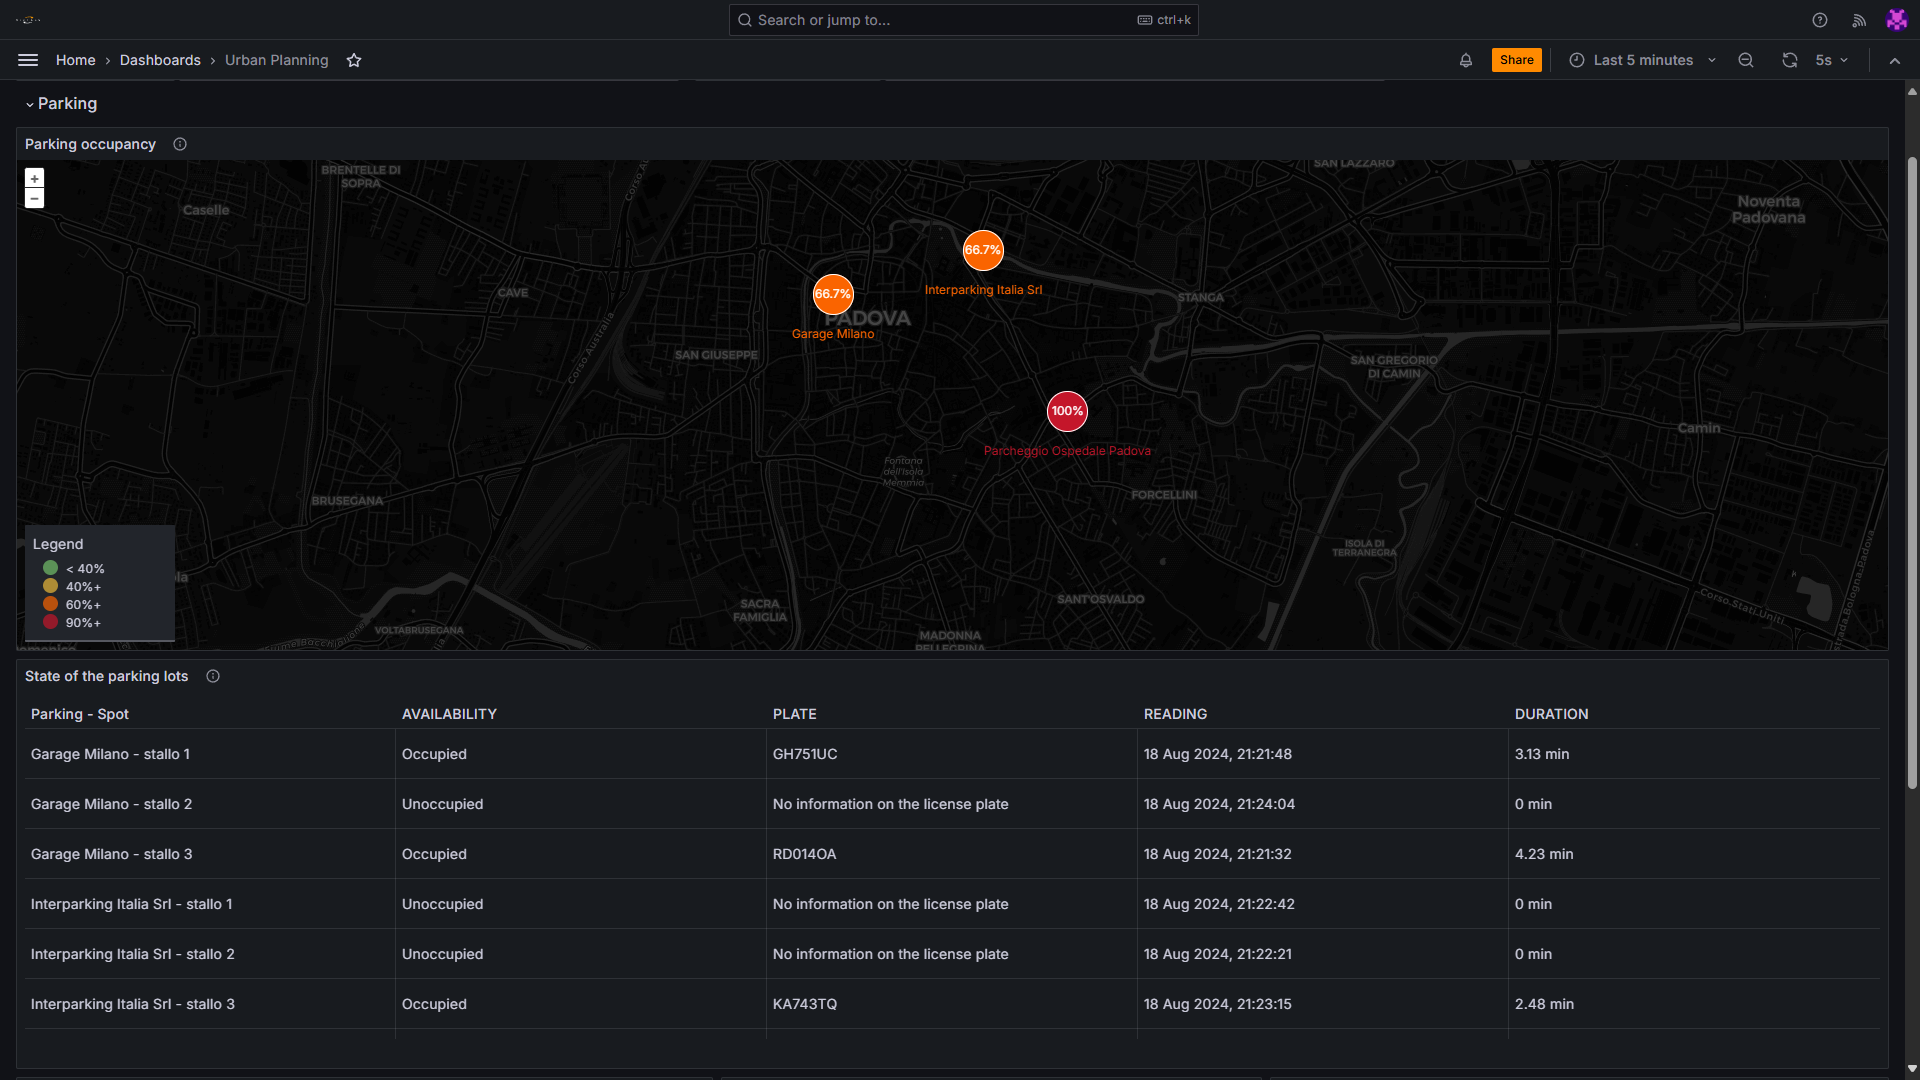
\includegraphics[width=15cm]{images_mu/parking1.png}
    \caption{Prima parte pannelli relativi ai parcheggi.}
    \label{fig:Prima parte pannelli relativi ai parcheggi.}
\end{figure}
\begin{figure}[H]
    \centering
    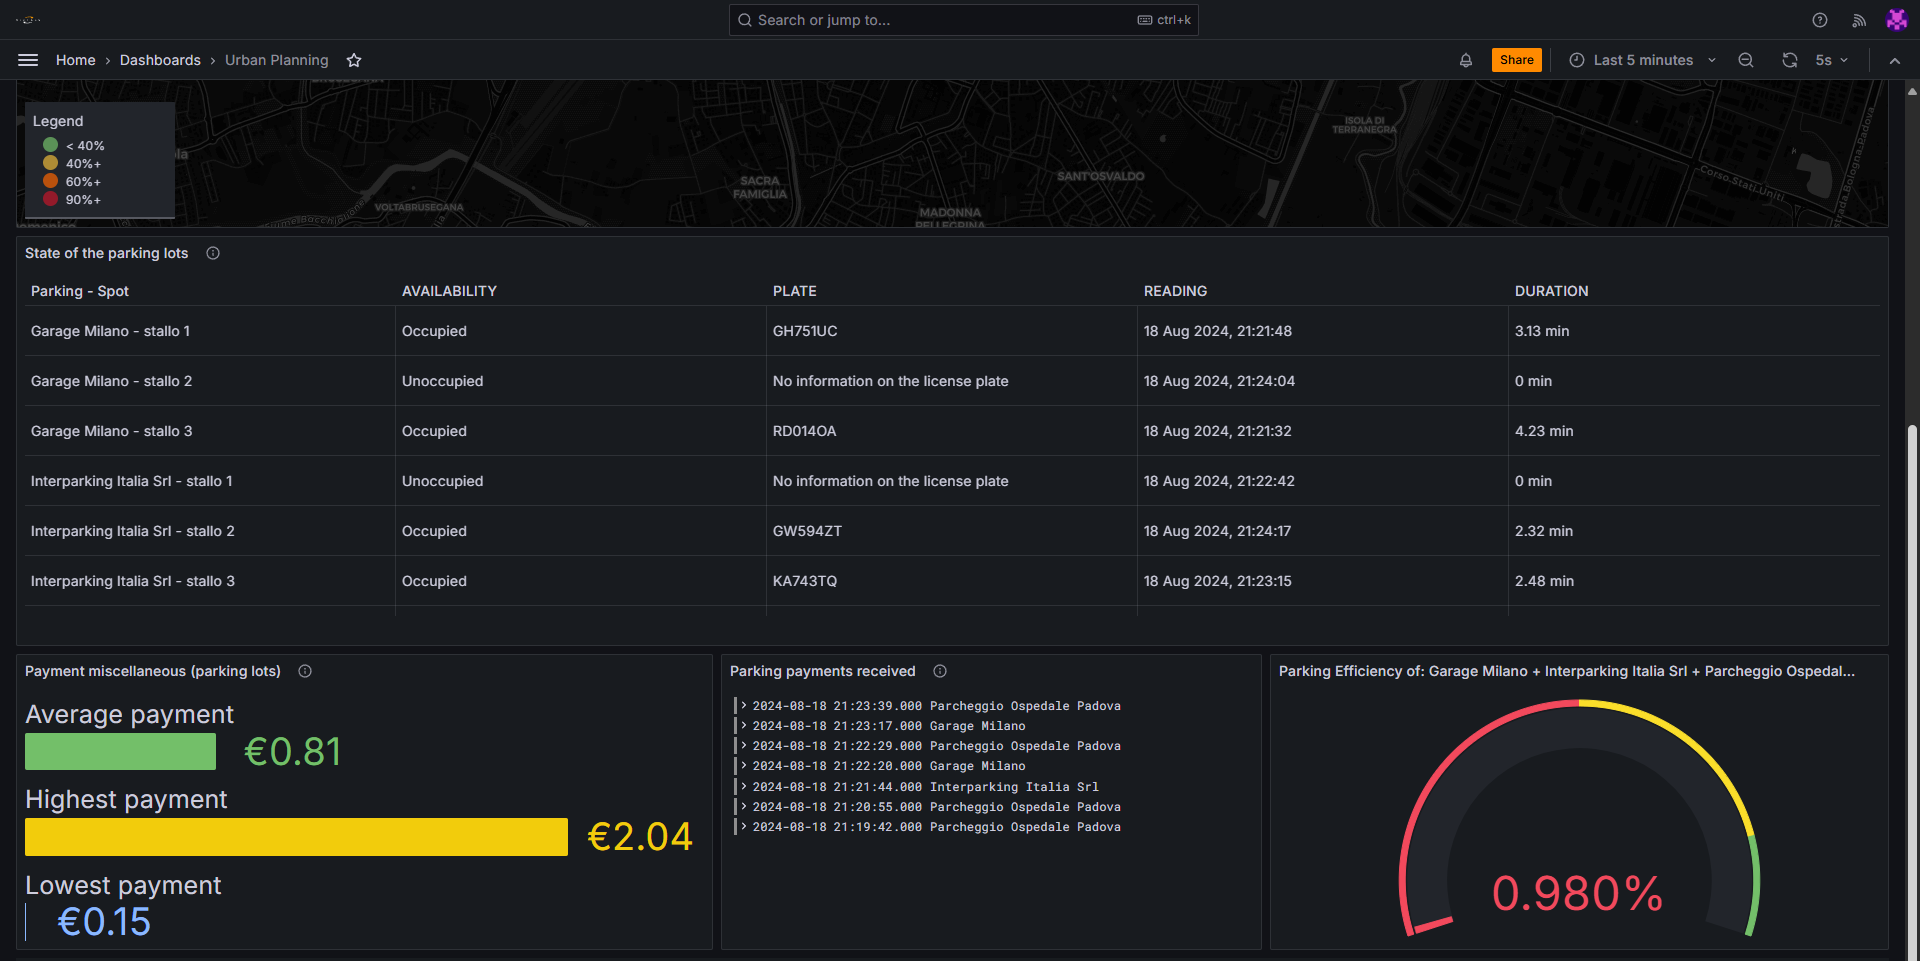
\includegraphics[width=15cm]{images_mu/parking2.png}
    \caption{Seconda parte pannelli relativi ai parcheggi.}
    \label{fig:Seconda parte pannelli relativi ai parcheggi.}
\end{figure}
\subsubsection{Colonnine di ricarica}
\begin{itemize}
\setlength\itemsep{0em}
    \item Mappa che indica la percentuale di colonnine di ricarica occupate all'interno delle aree di sosta;
    \item Tabella contenente le informazioni sullo stato delle singole colonnine. In particolare, per ciascuna di esse si riportano lo stato (libera o occupata) e, in caso di occupazione, la targa dell'auto attualmente collegata, l'orario di inizio e la durata della ricarica;
    \item Ortogramma a nastro con le statistiche dei pagamenti ricevuti. In particolare, il pannello mostra il costo minimo e massimo delle ricariche avvenute, oltre al costo medio;
    \item Pannello Log contenente le informazioni di tutti i pagamenti ricevuti;
    \item Pannello Time series che mostra l'andamento nel tempo dei consumi di energia elettrica dovuti alle ricariche dei veicoli.
\end{itemize}
\begin{figure}[H]
    \centering
    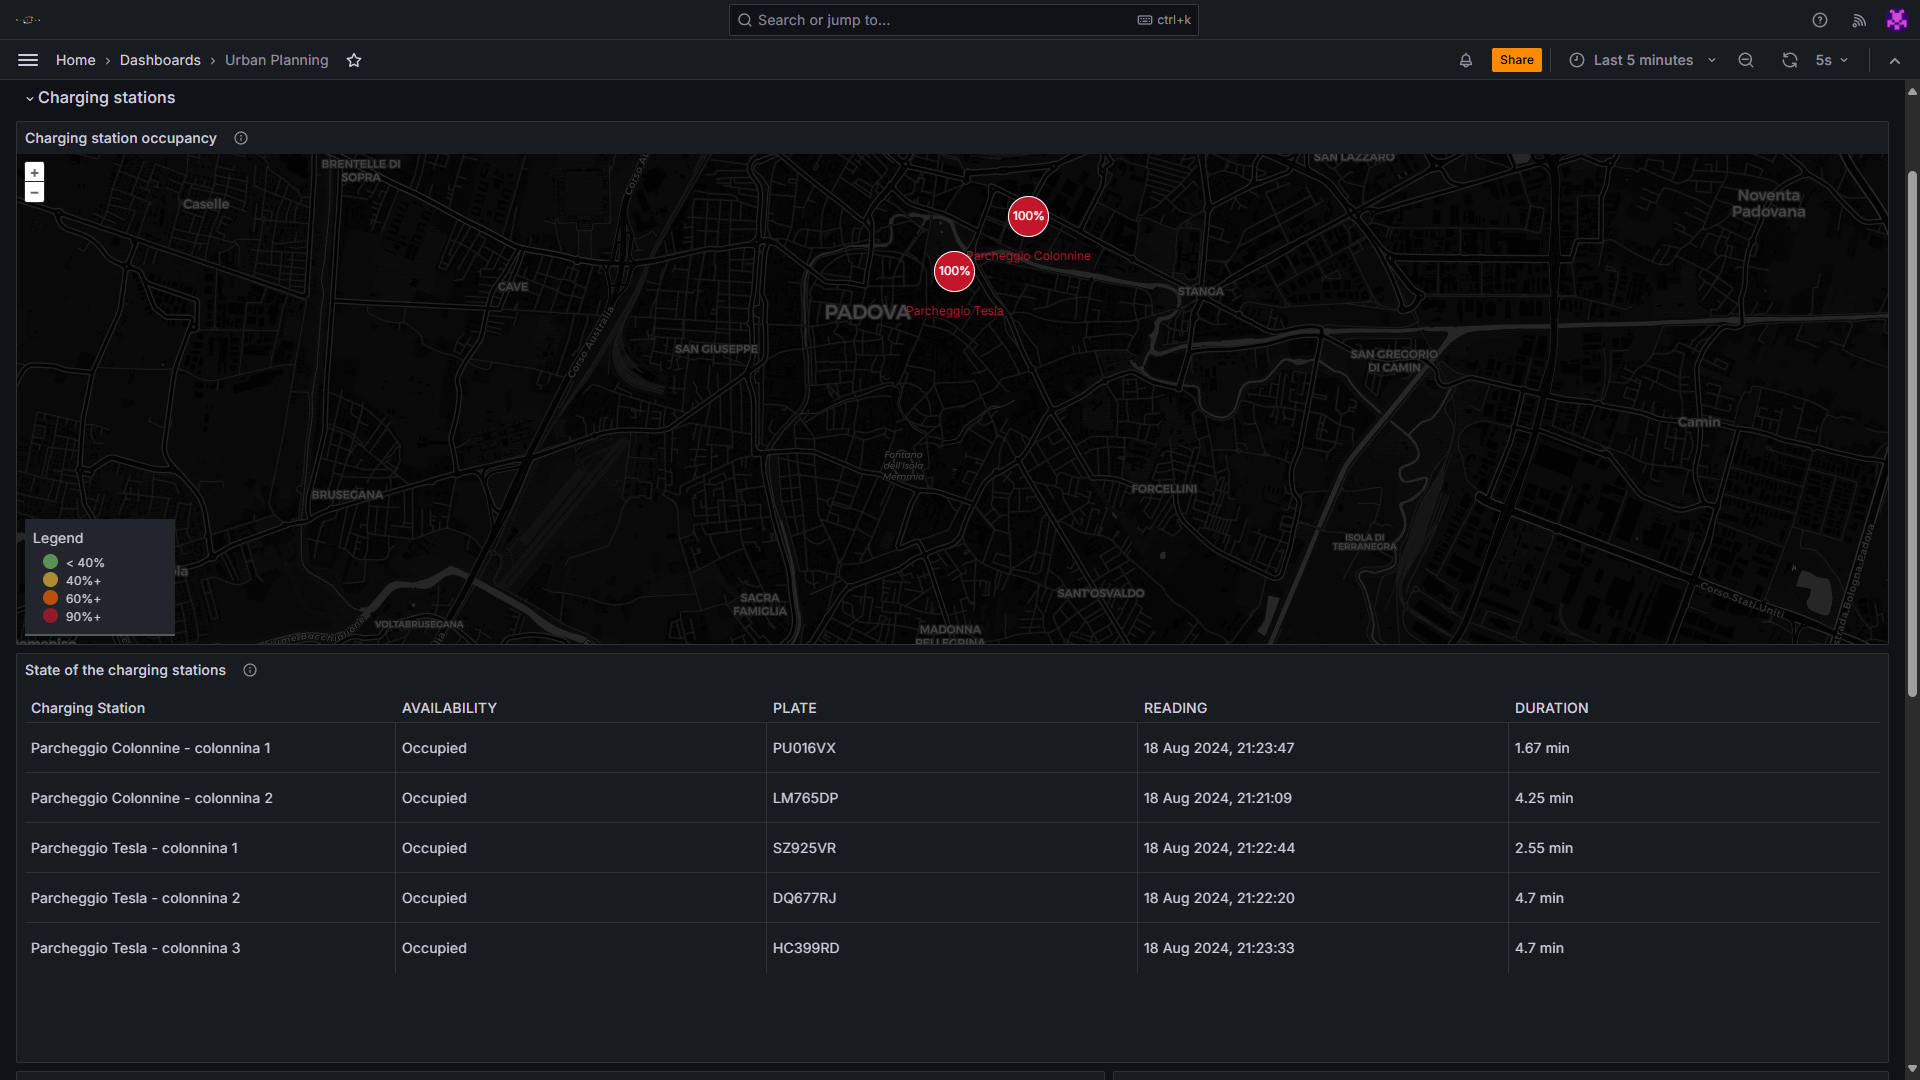
\includegraphics[width=15cm]{images_mu/charging_station1.png}
    \caption{Prima parte pannelli relativi alle colonnine di ricarica.}
    \label{fig:Prima parte pannelli relativi alle colonnine di ricarica.}
\end{figure}
\begin{figure}[H]
    \centering
    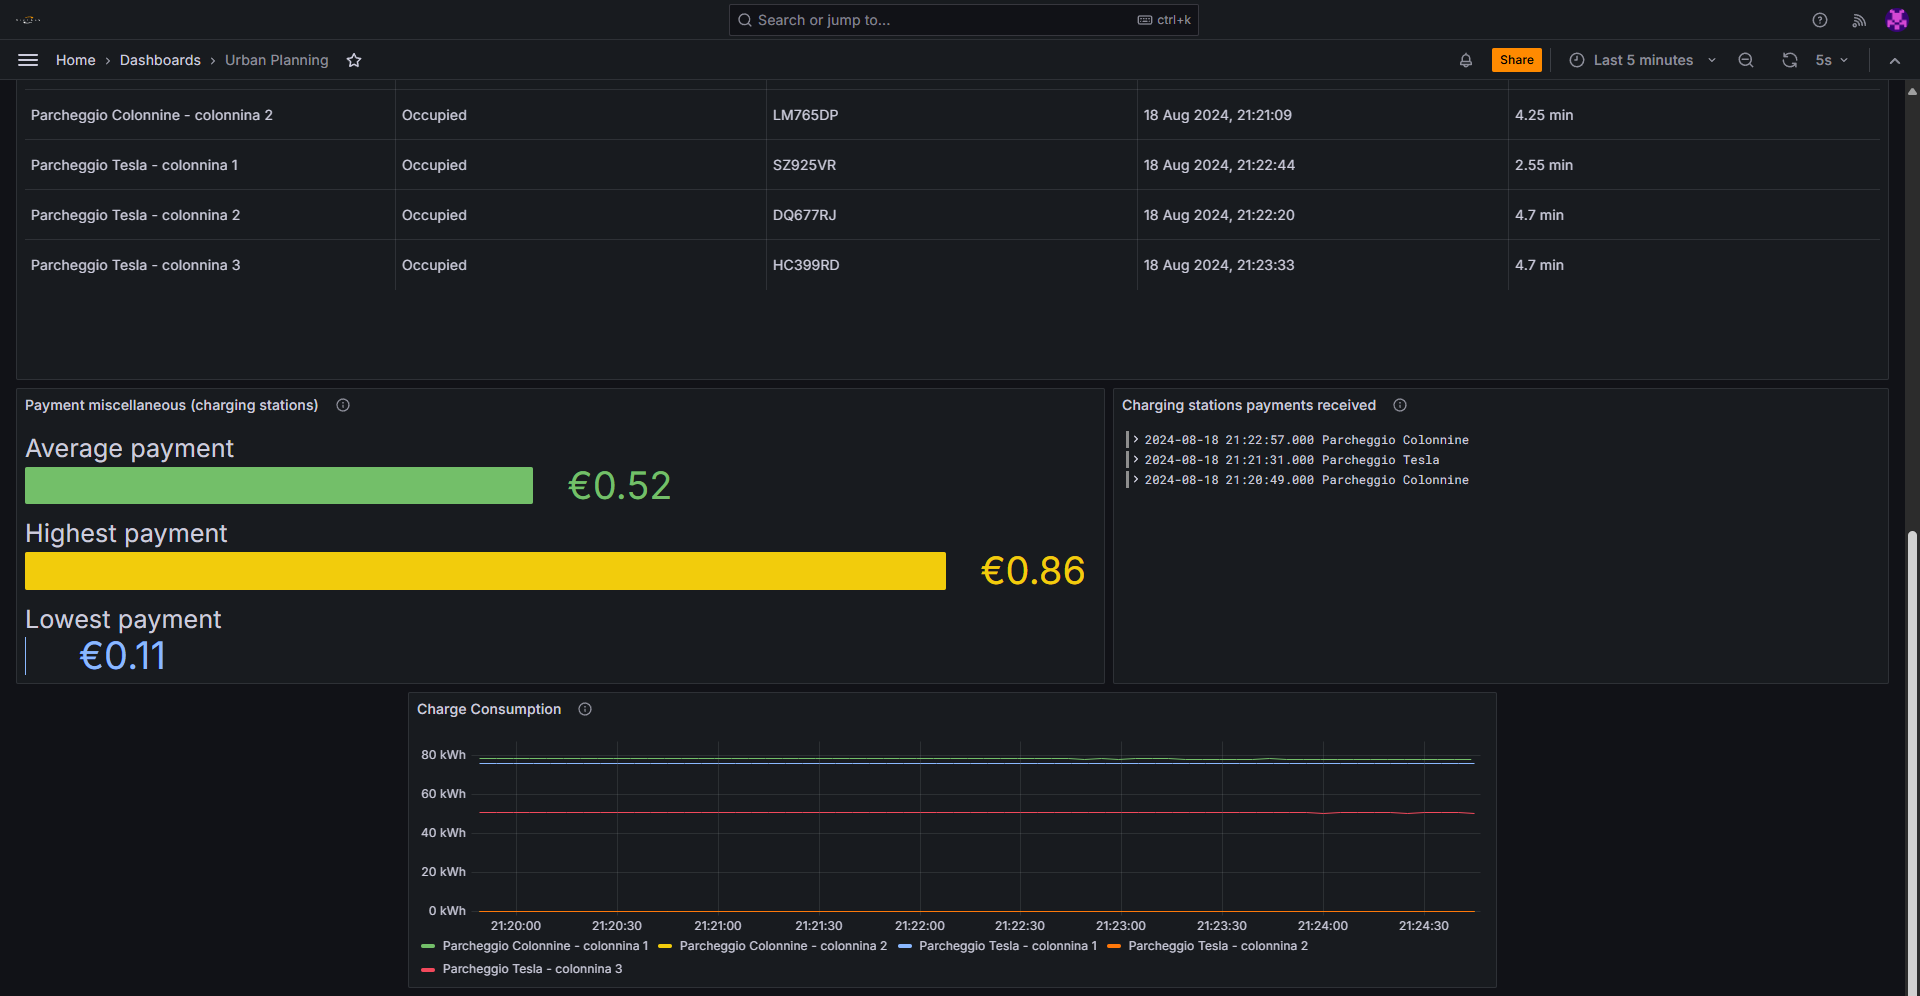
\includegraphics[width=15cm]{images_mu/charging_station2.png}
    \caption{Seconda parte pannelli relativi alle colonnine di ricarica.}
    \label{fig:Seconda parte pannelli relativi alle colonnine di ricarica.}
\end{figure}
\subsubsection{Riempimento isole ecologiche}
\begin{itemize}
\setlength\itemsep{0em}
    \item Grafico a linee che mostra l'andamento nel tempo del livello di riempimento dei conferitori delle isole ecologiche.
\end{itemize}
\begin{figure}[H]
    \centering
    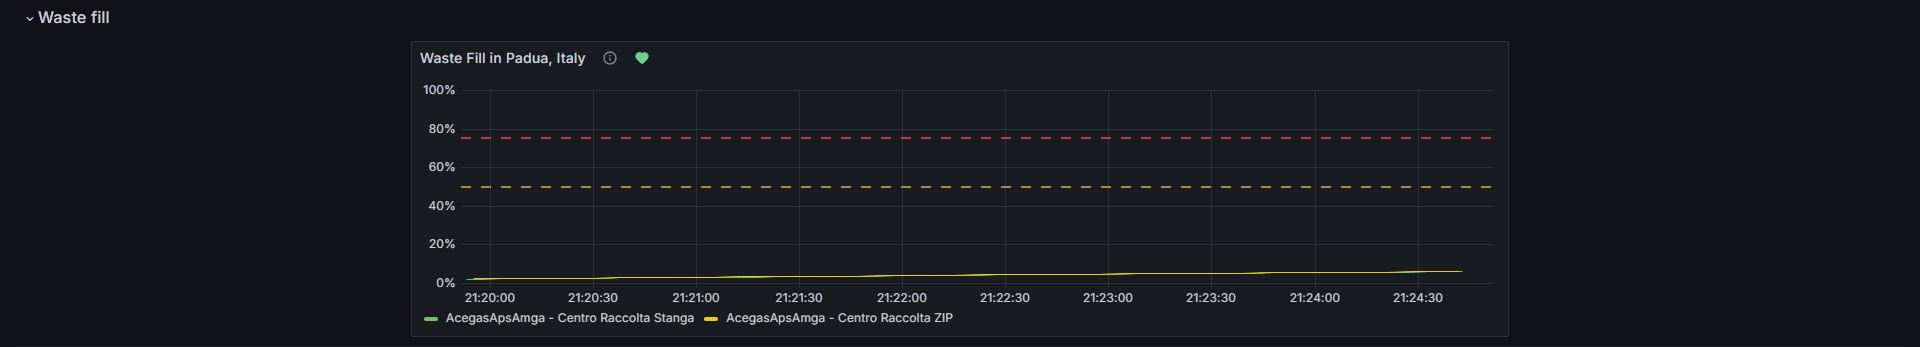
\includegraphics[width=15cm]{images_mu/waste_fill.png}
    \caption{Pannelli relativi al riempimento dei conferitori delle isole ecologiche.}
    \label{fig:Pannelli relativi al riempimento dei conferitori delle isole ecologiche}
\end{figure}
\subsubsection{Guasti elettrici}
\begin{itemize}
\setlength\itemsep{0em}
    \item Mappa che mostra la posizione delle centraline elettriche e il loro stato (funzionante o guasta).
\end{itemize}
\begin{figure}[H]
    \centering
    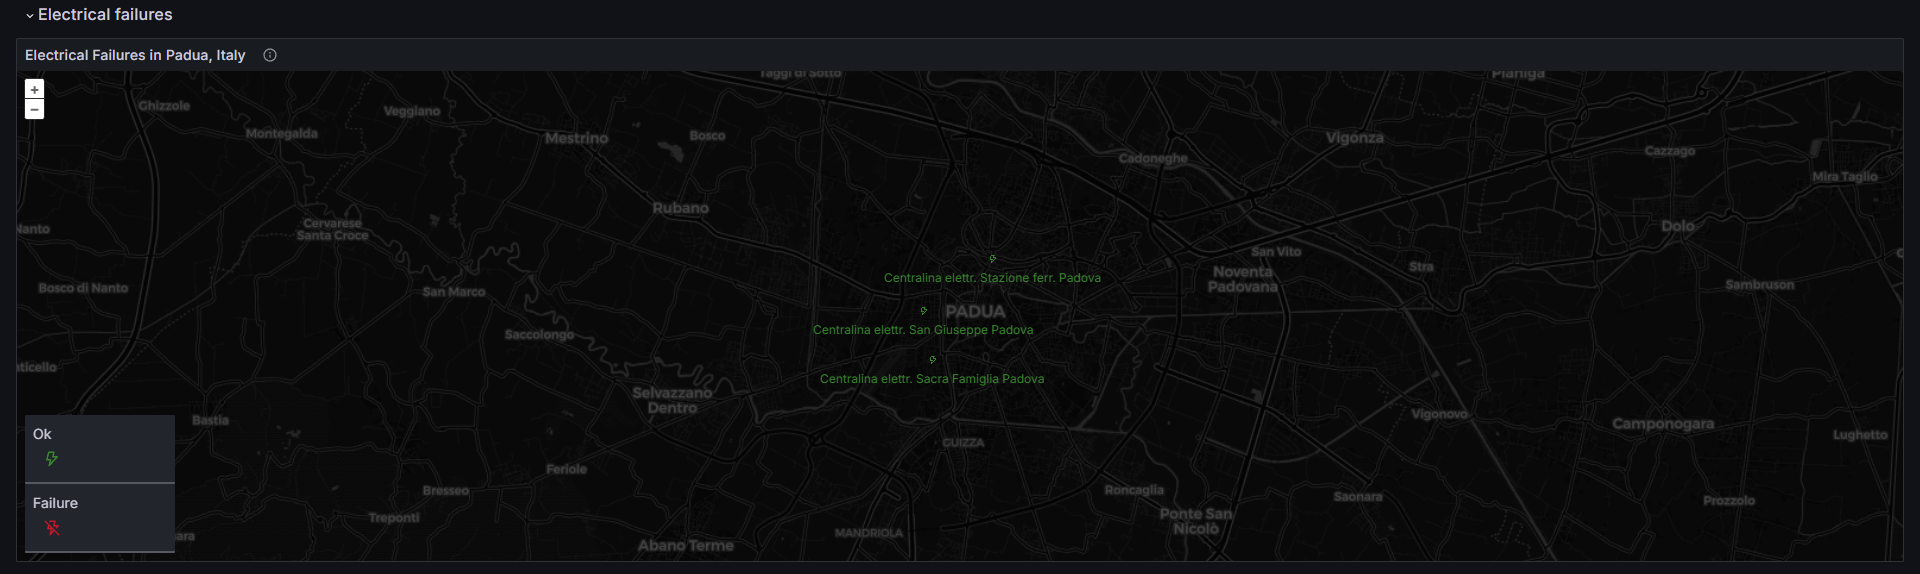
\includegraphics[width=15cm]{images_mu/electrical_failure.png}
    \caption{Pannelli relativi ai guasti elettrici.}
    \label{fig:Pannelli relativi ai guasti elettrici}
\end{figure}
\subsection{Dashboard ``Superamento Soglie"} \label{sec:thresholds}
La dashboard ``Exceeding Thresholds" consente di visualizzare i dati relativi al superamento delle soglie di sicurezza di alcune misurazioni, quali temperatura percepita, intensità delle precipitazioni, inquinamento atmosferico, livello di riempimento dei bacini idrici e livello di riempimento dei conferitori nelle isole ecologiche. Per ciascuna di queste tipologie di rilevazione, è presente un pannello contenente una lista di allerte. Le notifiche vengono inviate all'utente quando i valori misurati dai sensori superano le soglie impostate. La dashboard funge da storico delle notifiche ricevute e i vari pannelli al suo interno consentono di avere una visione panoramica e sintetica dello stato delle allerte. I widget sono suddivisi in due righe, uno per ciascuna area di interesse, contenenti da uno a più pannelli. Alle sezioni seguenti viene illustrato il contenuto di ciascuna riga, per maggiori informazioni sul funzionamento delle notifiche si rimanda alla sezione \ref{sec:alert}.
\subsubsection{Dominio ambientale}
Contiene i pannelli in formato ``Alert list" relativi alle seguenti misurazioni:
\begin{itemize}
\setlength\itemsep{0em}
    \item Temperatura percepita;
    \item Intensità delle precipitazioni;
    \item Inquinamento dell'aria;
    \item Livello dell'acqua.
\end{itemize}
\begin{figure}[H]
    \centering
    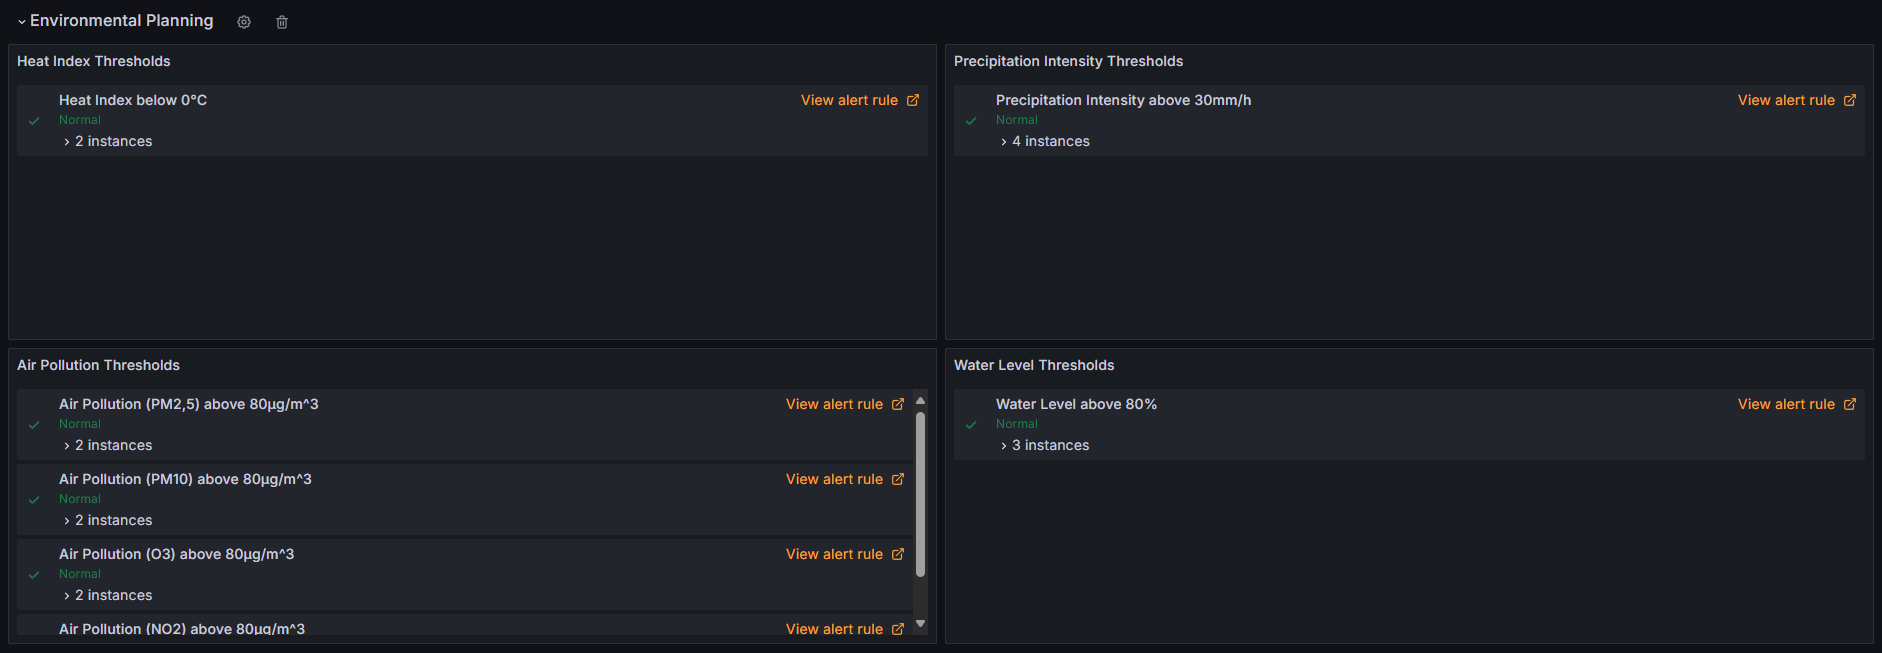
\includegraphics[width=15cm]{images_mu/environmental_thresholds.png}
    \caption{Pannelli relativi alle notifiche del dominio ambientale.}
    \label{fig:Pannelli relativi alle notifiche del dominio ambientale}
\end{figure}
\subsubsection{Dominio urbanistico}
Contiene un unico pannello relativo al riempimento dei conferitori delle isole ecologiche.
\begin{figure}[H]
    \centering
    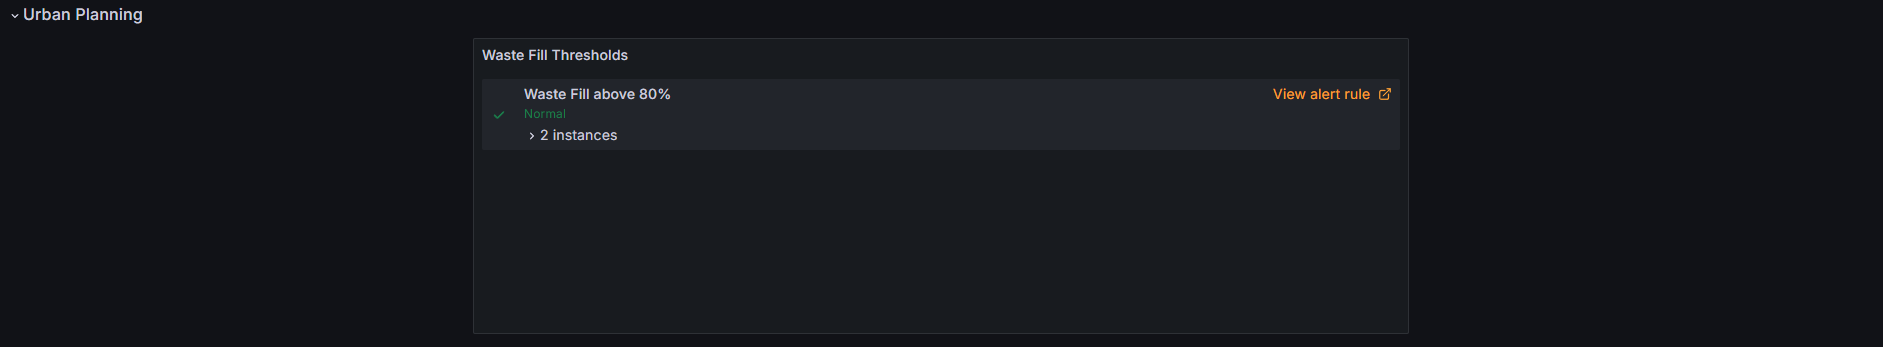
\includegraphics[width=15cm]{images_mu/urban_thresholds.png}
    \caption{Pannelli relativi alle notifiche del dominio urbanistico}
    \label{fig:Pannelli relativi alle notifiche del dominio urbanistico}
\end{figure}
\subsection{Allerte} \label{sec:alert}
L'applicativo è dotato di un sistema di notifica, funzionalità che consiste, per l'appunto, nell'invio di notifiche all'utente qualora i valori misurati da alcune tipologie di sensori (descritti alla sezione \ref{sec:thresholds}) superassero le soglie di sicurezza impostate. L'utente viene dunque tempestivamente avvisato di eventuali criticità o eventi pericolosi, in modo da poter intraprendere strategie mitigative il prima possibile. L'utente può visualizzare le impostazioni del sistema di notifica alla pagina ``Alerting". \\ I messaggi di notifica vengono inviati via mail e sull'apposito server \glossterm{Discord}, configurato dall'amministratore di sistema. All'interno dell'applicazione vi è anche una dashboard panoramica sullo stato delle allerte, anch'essa illustrata alla sezione \ref{sec:thresholds}.
\begin{figure}[H]
    \centering
    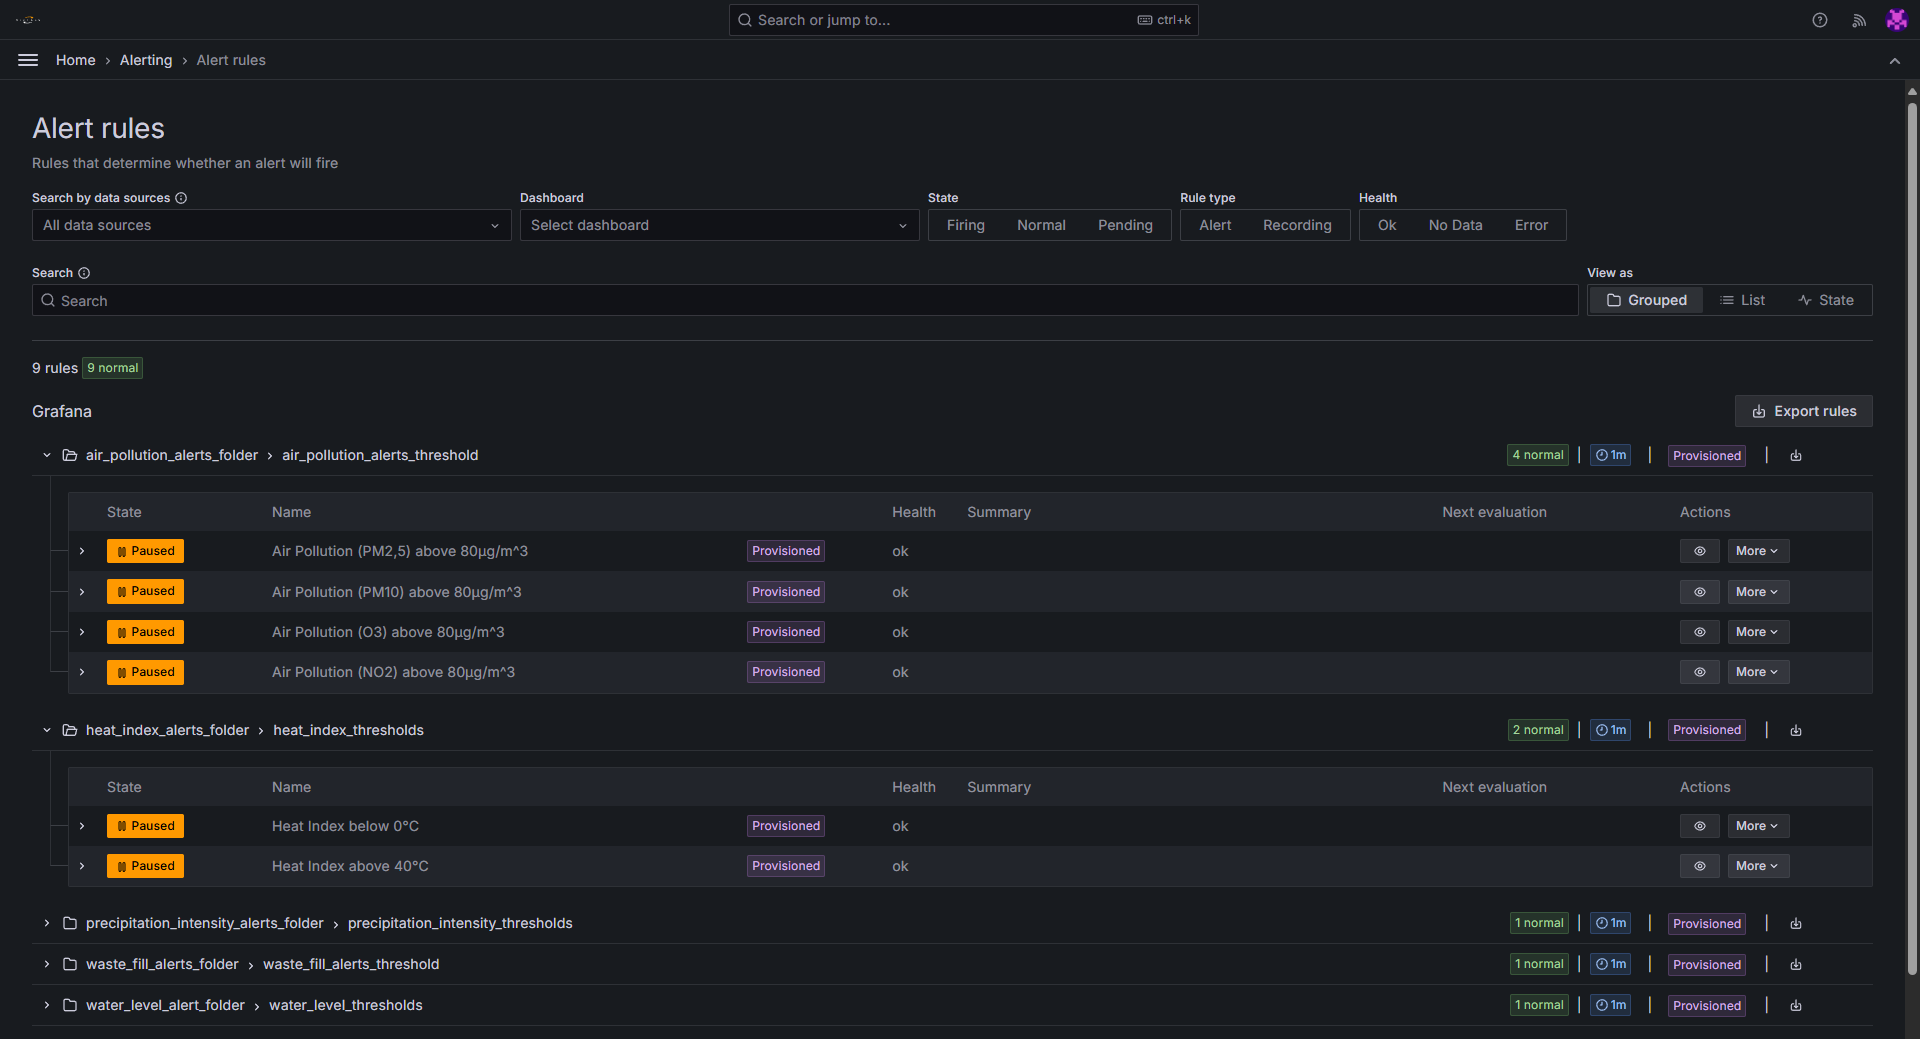
\includegraphics[width=15cm]{images_mu/alerting.png}
    \caption{Alcuni esempi di alert rules.}
    \label{fig:Alcuni esempi di alert rules}
\end{figure}
\begin{figure}[H]
    \centering
    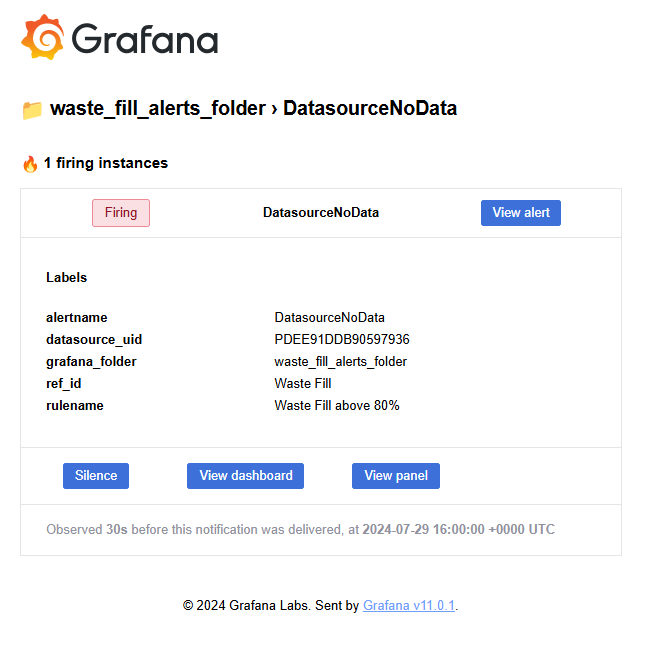
\includegraphics[width=9cm]{images_mu/mail.png}
    \caption{Esempio di mail inviata dal sistema di notifica.}
    \label{fig:Esempio di mail inviata dal sistema di notifica}
\end{figure}
\begin{figure}[H]
    \centering
    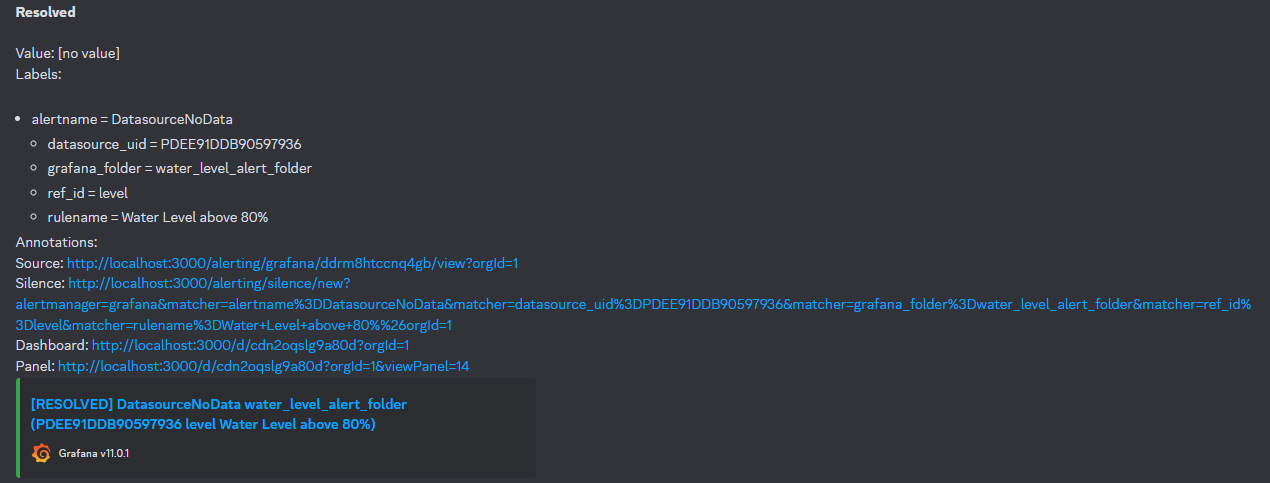
\includegraphics[width=15cm]{images_mu/discord.png}
    \caption{Esempio di messaggio inviato su Discord dal sistema di notifica.}
    \label{fig:Esempio di messaggio inviato su Discord dal sistema di notifica}
\end{figure}
\section{Supporto tecnico} \label{sec:support}
Per assistenza tecnica relativa all’utilizzo del prodotto software SyncCity, viene fornito il
seguente indirizzo email:
\begin{center}
    \parbox{\linewidth}{\centering
        \href{mailto: nan1fyteam.unipd@gmail.com}{nan1fyteam.unipd@gmail.com}
    }
\end{center}
Si è gentilmente pregati di includere nel corpo dell’email una descrizione quanto più completa del problema riscontrato, 
insieme ad eventuali istantanee o dettagli aggiuntivi che possano aiutare la comprensione del problema e la risoluzione dello stesso.
Si invita, inoltre, a descrivere eventuali passaggi già tentati, in modo che il team possa fornire un’assistenza più mirata.
\end{document}
